\documentclass[
  % die Schriftgröße - sollten Sie nicht ändern
  fontsize=12pt,
  % das Papierformat, also DIN A4
  paper=A4,
  % Literaturverzeichnis ins Inhaltsverzeichnis
  bibliography=totoc,
  % andere Verzeichnisse ebenfalls ins Inhaltsverzeichnis
  listof=totoc,
  % abgesetzte Formeln linksbündig
  fleqn,
  % für die Satzspiegelkonstruktion - siehe KOMA-Doku
  DIV=12,
  % Bindekorrektur (linker Rand) - evtl. anpassen
  BCOR=1mm,
  % die im Text verwendeten Sprachen (u.a. für das Paket babel); die
  % letztgenannte (!) Sprache ist die Standardsprache; "n"german steht für die
  % neue Rechtschreibung
  english,ngerman,
  % weil (s.u.) das Paket geometr verwendet wird
  usegeometry,
  % wie Absätze gesetzt werden: ohne Einzug, halbe Zeile Abstand
  parskip=half-
]{scrreprt}


%Versuch eine Grafik zu erstellen
\usepackage[dvipsnames,table]{xcolor}
\usepackage{siunitx}
\usepackage{pgf-spectra}
\usepackage{pgfplots}
\pgfplotsset{compat=newest}
  \pgfplotsset{plot coordinates/math parser=false}
  \newlength\figureheight
  \newlength\figurewidth

%% the following commands are needed for some matlab2tikz features
\usetikzlibrary{plotmarks}
\usetikzlibrary{arrows.meta}
\usepgfplotslibrary{patchplots}
\usepackage{grffile}
\usepackage{amsmath}
\usepackage{matlab-prettifier}

\usepackage{float}

\usepackage{graphicx}
\usepackage{subcaption}
%Zum Zentrieren von Tabellen-Captions
\usepackage[justification=centering]{caption}

% Beschriftungen für Tabellen kommen linksbündig über die Tabelle
\KOMAoption{captions}{tableheading,nooneline}
\setcaptionalignment[figure]{c}
\setcaptionalignment[table]{l}

%Für das einbinden von Code
\usepackage{listings}
\lstset{numbers=left, numberstyle=\tiny, numbersep=5pt}
\lstset{language=Perl}

% wird für die Titelseite benötigt
\usepackage{geometry}

% wird für die Nutzung der Hausschrift benötigt
\usepackage{fontspec}
\usepackage[font=scriptsize]{caption}
\usepackage{mwe}

% Standardpaket für Lokalisation, siehe Option "ngerman" oben
\usepackage{babel}
% Laden von optimierten Trennmustern
\babelprovide[hyphenrules=ngerman-x-latest]{ngerman}

% Standardpaket für mathematische Zusatzfunktionen; wenn Sie keine
% mathematischen Formeln brauchen, können Sie diese Zeile löschen
\usepackage{amsmath}
\usepackage{amssymb}
\usepackage{trfsigns}
\usepackage{mathtools}
% die Hauptschrift Libertinus
\usepackage{libertinus-otf}
% die "Schreibmaschinenschrift" Anonymous Pro, angepasst
\usepackage{AnonymousPro}
\setmonofont{AnonymousPro}[Scale=MatchLowercase,FakeStretch=0.85]

% etwas größerer Zeilenabstand als im Buchsatz
\linespread{1.1}

% Paket für Feinkorrekturen an der Typographie, das für ein ausgewogeneres
% Schriftbild sorgt
\usepackage{microtype}

% Paket für kontextsensitive Anführungszeichen
\usepackage{csquotes}
% Shortcut, damit aus dem eigentlich falschen Zeichen " richtige
% Anführungszeichen je nach Sprache werden
\MakeOuterQuote{"}

% Paket, das den Befehl \includegraphics ermöglicht
\usepackage{graphicx}

% komfortablere Aufzählungen als in Standard-LaTeX; ein Beispiel findet man in
% chap3.tex
\usepackage{enumitem}

% Paket für mehr als die üblichen Standardfarben
\usepackage[dvipsnames]{xcolor}
% Definition der "Hausfarben" der HAW
\definecolor{haw}{HTML}{003CA0}
\definecolor{haw2}{HTML}{0096D2}
\definecolor{haw3}{HTML}{A0BEDC}

% typographisch anspruchsvolle Tabellen; siehe chap3.tex
\usepackage{booktabs}

% zum Erstellen des Literaturverzeichnisses; der gängige Stil APA ist hier
% bereits eingestellt
\usepackage[style=ieee]{biblatex}
% eine Beispieldatei für ein Literaturverzeichnis
\addbibresource{bib.bib}

% für die Erzeugung der Grafiken in chap3.tex; wenn Sie PGF/TikZ nicht
% verwenden wollen, können Sie diese Zeilen entfernen
\usepackage{tikz}
% Zusatzbibliotheken für TikZ, die in den genannten Beispielen verwendet
% werden
\usetikzlibrary{calc,intersections,angles,3d}

% für die Erzeugung des Codeblocks in chap3.tex; wenn in Ihrer Arbeit keine
% Codeblöcke vorkommen, können Sie diese Zeilen entfernen
\usepackage{listings}
% Anpassung des Erscheinungsbildes des Codeblocks; mehr dazu in der
% Dokumentation des Pakets "listings"
\lstdefinestyle{mystyle}{
    backgroundcolor=\color{gray!20},
    keywordstyle=\color{haw2},
    numberstyle=\footnotesize\color{haw},
    basicstyle=\ttfamily\small,
    captionpos=t,
    frame=single,
    framerule=0pt,
    keepspaces=true,
    numbers=left,
    numbersep=6pt,
    belowcaptionskip=1em,
    aboveskip=\bigskipamount,
}
\lstset{style=mystyle}
% damit es "Codeblock" und nicht "Listing" heißt
\renewcommand{\lstlistingname}{Codeblock}

% für die Verlinkung innerhalb des PDF-Dokuments, für PDF-Lesezeichen und
% PDF-Metadaten; dieses Paket sollte üblicherweise immer als letztes geladen
% werden
\usepackage[colorlinks=false,allcolors=black,hyperfootnotes=false,pageanchor=true,linktoc=all]{hyperref}

% für die Druckversion können Sie die obige Zeile durch die folgende ersetzen,
% damit Links nicht blau dargestellt werden:
%\usepackage[draft]{hyperref}

% Metadaten des PDF-Dokumentes; setzen Sie hier Ihren eigenen Namen sowie den
% Titel Ihrer Arbeit ein
\hypersetup{pdfauthor={Magnus Müller, Steffen Sterthoff, Darius Daub}}
\hypersetup{pdftitle={SPT Inselnetz}}




\newcommand{\norm}[1]{\left\lVert#1\right\rVert}

\DeclareMathAccent{\ring}%
    {\mathalpha}{operators}{"17}
\providecommand*{\angs}%
    {\ensuremath{\smash{\mathrm{\ring A}}}}
\providecommand*{\ohm}%
    {\ensuremath{\mathrm{\Omega}}}
\providecommand*{\degree}%
    {\ensuremath{^\circ}}
\providecommand*{\celsius}%
    {\ensuremath{\mathrm{^\circ C}}}
\providecommand*{\micro}%
    {\ensuremath{\mu}}
\providecommand*{\unit}[1]{%
    \ensuremath{\mathrm{\,#1}}}
% The number `e'
\providecommand*{\eu}%
    {\ensuremath{\mathrm{e}}}
% The imaginary unit
\providecommand*{\iu}%
    {\ensuremath{\mathrm{j}}}
\providecommand*{\ped}[1]{%
    \ensuremath{_\mathrm{#1}}}
\providecommand*{\ap}[1]{%
    \ensuremath{^\mathrm{#1}}}
\providecommand{\newoperator}[3]{%
    \newcommand*{#1}{\mathop{#2}#3}}
\providecommand{\renewoperator}[3]{%
    \renewcommand*{#1}{\mathop{#2}#3}}
\newoperator{\ent}%
    {\mathrm{ent}}{\nolimits}
\renewoperator{\Re}%
    {\mathrm{Re}}{\nolimits}
\renewoperator{\Im}%
    {\mathrm{Im}}{\nolimits}
\makeatletter
\providecommand*{\diff}%
    {\@ifnextchar^{\DIfF}{\DIfF^{}}}
\def\DIfF^#1{%
    \mathop{\mathrm{\mathstrut d}}%
    \nolimits^{#1}\gobblespace}
    \def\gobblespace{%
    \futurelet\diffarg\opspace}
\def\opspace{%
    \let\DiffSpace\!%
    \ifx\diffarg(%
    \let\DiffSpace\relax
    \else
    \ifx\diffarg[%
    \let\DiffSpace\relax
    \else
    \ifx\diffarg\{%
    \let\DiffSpace\relax
    \fi\fi\fi\DiffSpace}
\providecommand*{\deriv}[3][]{%
    \frac{\diff^{#1}#2}{\diff #3^{#1}}}
\providecommand*{\pderiv}[3][]{%
    \frac{\partial^{#1}#2}%
    {\partial #3^{#1}}}

\usepackage[headsepline,automark]{scrlayer-scrpage}

% Kopf- und Fußzeilen ------------------------------------------------------
\pagestyle{scrheadings}
    
% Kopf- und Fußzeile auch auf Kapitelanfangsseiten -------------------------
\renewcommand*{\chapterpagestyle}{scrheadings}
    
% Schriftform der Kopfzeile ------------------------------------------------
\renewcommand{\headfont}{\normalfont}
    
% Kopfzeile ----------------------------------------------------------------
\ihead{
    \parbox{11.8cm}{\normalsize{ \ }}\\
    %\small{\untertitel}\\[2ex]
    \textit{ \headmark}
}
\chead{
        %\includegraphics[height=0.8cm]{Grafiken/EWENETZ_Logo.png}
}
\ohead{	
        
\includegraphics[height=1.4cm]{Abbildungen/Logo_HSB_Hochschule_Bremen.png}	
}
\setlength{\headheight}{21mm} % Höhe der Kopfzeile
    
\usepackage{pdfpages}

\begin{document}
\begin{titlepage}
    % andere Seitenränder als im Rest der Arbeit
    \newgeometry{lmargin=2cm,tmargin=7mm,rmargin=5mm,bmargin=1cm}
    % die "Hausfarbe" der HAW; diese und die folgenden Einstellungen sind lokal
    % und gelten nur innerhalb der Umgebung "titlepage"
    \color{haw}
    % Blocksatz für die Titelseite deaktivieren
    \raggedright
    % Logo rechtsbündig setzen
    \hfill
\includegraphics[width=7cm]{HSB.png}\\
  
    % vertikaler Abstand
    \vspace{5cm}
  
    % Wahl der "Hausschrift" Open Sans der HAW, die als Schrift auf Ihrem
    % Rechner installiert sein muss
    \setmainfont{Open Sans}
    % etwas kleiner als üblich
    \small
    % fett und in Majuskeln
    \textbf{DOKUMENTATION}
  
    % vertikaler Abstand
    \vspace{8mm}
  
    % der Titel der Arbeit als "Seite in der Seite"; natürlich müssen Sie hier
    % Ihren Titel eintragen
    \begin{minipage}{0.8\linewidth}
      % Wahle der zweiten "Hausschrift" der HAW, die ebenfalls auf Ihrem Rechner
      % bereits vorhanden sein muss
      % ziemlich große Schrift
      \LARGE
      % [1mm] steht jeweils für einen etwas größeren Durchschuss
      AUFGABE 3:\\[1mm]
      Simulation einer Gleichstrommaschine\\[1mm]
      % am Ende noch ein waagerechter Strich, das CD will es so...
      \,\rule{11mm}{1.2mm}
    \end{minipage}
  
    % vertikaler Abstand, überraschenderweise
    \vspace{1cm}
  
    % hier korrektes Datum und Ihren Namen eingeben
    Dezember 2023\\
    Farshid Abdehgah \\
    Darius Daub
  
    % letzter vertikaler Abstand für heute
    \vspace{5cm}
  
    % noch eine "Seite in der Seite", etwas nach rechts geschoben
    \hspace*{37mm}
    \begin{minipage}{0.5\linewidth}
      % Namen und Titel der beiden Prüfer eintragen
      \begin{tabular}{@{}l}
        Lehrender: Prof.\ Dr.\ Christian Mehler \\
        Anwendungen der Leistungselektronik  \\
        Master Energietechnik \\
      \end{tabular}\\
  
      % noch ein horizontaler Strich
      \,\rule{9mm}{1mm}\\[1.5mm]
  
      \textbf{HOCHSCHULE BREMEN}\\
      \textbf{CITY UNIVERSITY OF APPLIED SCIENCES}\\
      Fakultät Natur und Technik\\
      Abteilung Maschinenbau\\
    \end{minipage}
  \end{titlepage}
  % setzt die Geometrie wieder auf die Standardwerte zurück
  \restoregeometry
  % für die Seite mit dem Abstract keine Seitenzahl ausgeben
  \thispagestyle{empty}
  
\tableofcontents
\thispagestyle{empty}
\chapter{Einleitung}
\chapter{Theoretische Grundlagen}

\section{Verbraucher in Inselnetzen}

Der folgende Abschnitt befasst sich mit der Beschreibung der Stromverbraucher für das vorliegende Inselnetz. 
Für eine fiktive Kommune gibt es verschiedene Verbrauchertypen, welche es näher zu untersuchen gilt. 
Ziel dabei ist es, reale Verbraucher zu kategorisieren und ihren Verlauf genauer zu analysieren. 
Da der Fokus der Simulation auf dem Netz und Speichertechnologien liegt, werden Vereinfachungen zur Darstellung in MatLab/Simulink vorgenommen.
Die Betrachtung potentieller Verbraucher und ihre Modellierung in einem Inselnetz-Modell wird in den folgenden beiden Abschnitten genauer analysiert. 
Im ersten Schritt wird die momentane Situation in Deutschland und seinen Kommunen hinsichtlich Differenzierung und Verbrauch beschrieben. 
Danach erfolgt die Ermittlung eines Konzepts zur Abschätzung von Verbräuchen mittels Lastkurven. 
Ziel der Unterteilung ist zuerst einen Überblick über die Basis des zu modellierenden Inselnetzes zu schaffen. 
Danach gilt es daraus pauschale Verbräuche unter Einbezug von Lastkurven zu ermitteln, welche in MatLab/Simulink simulationstauglich sind.

\subsecction(Verbraucher am Stromnetz)

Die potentiell zu betrachtenden Verbraucher für das Inselnetz entsprechen dabei denen einer deutschen Kommune am deutschen Stromnetz. 
Sie werden dabei in verschiedene Kategorien unterteilt und in folgenden Sub-Abschnitten genauer analysiert. 
Dabei erfolgt eine Differenzierung in Wohngebäude (WG), Nichtwohngebäude (NWG), die Interaktion dieser beiden Verbraucher mit eigenen Speichern, Windkraft und PV-Anlagen im Unterpunkt „Prosumer“, der Faktor Elektromobilität und weitere Verbraucher, die noch nicht betrachtet wurden. 
Die für das Inselnetz relevanten Parameter sind hierbei der Stromverbrauch und das Lastprofil jeden Verbrauchers, sowie deren Vorkommen in einer durchschnittlichen, deutschen Kommune. 
Außerdem wird noch die Möglichkeit der Einspeisung von Strom in ein Fernwärmenetz bzw. die Umwandlung von Strom in Wasserstoff als Power-to-Gas beschrieben.

\subsubsection(Wohngebäude (WG))

In Deutschland gibt es etwa 19,5 Mio. Wohngebäude, die an das Stromnetz angebunden sind. Dabei hat jedes Wohngebäude einen Energieverbrauch, der sich aus verschiedenen Faktoren zusammensetzt. 
Diese lassen sich in Raumwärme, Warmwasser, Beleuchtung, Betrieb von Elektrogeräten und sonstiger Prozesswärme unterteilen. 

to do
Abbildung 1: Energieverbrauch WG 

Hierbei werden die Faktoren Elektrogeräte und Beleuchtung in der Regel durch Strom gedeckt. 
Die Faktoren Warmwasser und Raumwärme sind abhängig vom eingebauten Heizungssystem. 
Hierbei sind eine anteilige bis vollständige Erzeugung der Raumwärme und des Warmwassers durch eine strombetriebene Wärmepumpe, eine Stromheizung oder ein Wärmenetz möglich und für die Simulation relevant. 
Dabei ist zu beachten, dass insbesondere bei Wärmepumpen der Wärmeenergieverbrauch stark vom Strombedarf abweicht. 
Eine Umrechnung mit Hilfe der Jahresarbeitszahl (JAZ) ist möglich. 
Im Neubau liegt der Anteil der verbauten Wärmepumpen im Jahr 2022 bei ca. 57\%.

Die Höhe des Energieverbrauches ist außerdem abhängig von der Anzahl der Bewohner des Wohngebäudes und dessen Größe als auch Zustand. 
Im Gebiet Wohnen und Gebäude werden daher viele Annahmen und Hochrechnungen pro Kopf, pro Fläche oder pro Haushalt getätigt. Um die Verbraucher für verschiedene Simulationsszenarien vereinfacht zu ermitteln, wird hier wie im Folgenden beschrieben vorgegangen. 

to do
Abbildung 2: https://www.parbuilding.de/leitfaden-wohnungsbau/gebäudearten-wohnungstypen-bauweisen/typologie-für-wohngebäude/

Wohngebäude lassen sich generell noch in weitere Unterkategorien aufgliedern.
Dazu zählen Einfamilienhäuser, Mehrfamilienhäuser, große Mehrfamilienhäuser, Reihenhäuser, Hochhäuser und Doppelhaushälfte, sowie diverse Spezialfälle. 
Um die Simulation der Verbraucher simpel zu halten, werden zum Verbraucher „Einfamilienhaus“ auch energetisch in der gleichen Größenordnung liegende Wohngebäudetypen gezählt, beispielsweise Reihen- und Zweifamilienhäuser. 
Der Verbraucher „Mehrfamilienhaus“ umfasst äquivalent auch solche Wohngebäudetypen. 
Große Mehrfamilienhäuser (ab 13 Wohnungen), Hochhäuser und mittelgroße bis große Wohnheime werden in der Praxis dazugezählt. 
Diese werden nicht in der Simulation dargestellt.
Das liegt einerseits daran, dass es sich nicht um eine großstädtische Simulation handelt, andererseits daran, dass bei außergewöhnlich großen Wohngebäuden individuell stark abweichende Energieverbräuche – auch beim Stromverbrauch – entstehen. 
Der Einbezug dieser übersteigt die Komplexität dieses Aspektes der Simulation.
Unter Einbezug des Heizungssystems gilt es einen Gesamtenergieverbrauch des Verbrauchers zu ermitteln. 
Der Jahresverbrauch von Wohnenergie liegt pro Einfamilienhaus bei etwa 25.000 kWh. 
Mehrfamilienhäuser sind meist energieeffizienter was den Heizenergieverbrauch betrifft, jedoch hängt der Verbrauch stark von der Anzahl der Wohnfläche, Wohnungseinheiten und Bewohnern ab. 
Aus Simplifizierungsgründen wird hier mit dem bundesweiten Jahresenergieverbrauch pro Kopf gerechnet, 8.800 kWh. 
Bei der Annahme von durchschnittlich 12 Personen pro Mehrfamilienhaus entspricht dies einem Jahresenergieverbrauch von 105.600 kWh. 
Es wird angenommen, dass der Anteil vom Energieverbrauch sich zu 85\% auf das Heizen bezieht. 
Wenn man nun davon ausgeht, dass entweder eine Wärmepumpe oder ein anderes Heizungssystem verbaut ist, welches nicht auf Strom basiert, ergeben sich vier Szenarien. 
Bevor jedoch ein Stromverbrauch bei Nutzung einer Wärmepumpe errechnet werden kann, ist zu beachten, dass der Energieverbrauch durch den Wirkungsgrad der Wärmepumpe in Stromverbrauch umgerechnet werden muss. 
Dies über die Jahresarbeitszahl JAZ möglich. 
Bei dem am meisten verbauten Typ von Wärmepumpen, den Luft-Wasser-Wärmepumpen, liegt dieser üblicherweise im Bereich von 2 bis 4. 
Für die Berechnung wird mit einer JAZ von 3 gerechnet. Daher ergibt sich folgende Formel:

\begin{equation}
    \text{Strom pro Jahr} = \text{Enrg. pro Jahr} \times \frac{0.85}{3} + \text{Enrg. pro Jahr} \times 0.15
\end{equation}

Liegt keine Wärmepumpenheizung vor, wird der erste Teil des Terms gleich null gesetzt. 
Die vier resultierenden Verbrauchertypen werden in nachfolgender Tabelle aufgeführt, wobei aufgerundet wird:

\begin{table}[htbp]
    \centering
    \caption{Tabelle 1: 4 Szenarien (exakter Wert in den Klammern)}
    \label{tab:szenarien}
    \begin{tabular}{lccc}
        \toprule
        \textbf{Szenario/Verbrauch [kWh/a]} & \textbf{Einfamilienhaus} & \textbf{Mehrfamilienhaus} \\
        \midrule
        Heizung Wärmepumpe & 7,000 (7,083) & 30,000 (29,920) \\
        Heizung nicht abgebildet & 3,750 & 16,000 (15,840) \\
        \bottomrule
    \end{tabula

Der Momentanverbrauch wird durch Lastprofile abgeschätzt und im entsprechenden Abschnitt bearbeitet.

\subsubsection(Nichtwohngebäude (NWG))

Die Anzahl an Nichtwohngebäuden beläuft sich auf 21,5 Mio. in Deutschland, von denen 6 Mio. thermisch konditioniert sind. 
Diese lassen sich allgemein in Dienstleistungsgebäude, beispielsweise Schulen, Büros, Gastro, Sport und Produktionsgebäude, beispielsweise Werkstätten, Lager, Betriebe, unterteilen. 
Der Energieverbrauch allgemein und einhergehend der Stromverbrauch ist hierbei stark nutzungsabhängig. 
Während sich bei Dienstleistungsgebäuden die Verbrauchsfaktoren meist noch anteilig ähnlich derer bei Wohngebäuden verhalten, ist dies bei Produktionsgebäuden nicht der Fall. 
Dies geht soweit, dass eine Pauschalisierung der Verbrauchsaufschlüsselung nicht möglich ist.

abbildung hier 
Abbildung 3: Endenergieverbrauch nach Sektoren

Trotz deutschlandweit bekannter Gesamtverbräuche ist der Energiebedarf in einer Kommune stark von lokalen Gewerbegebieten und einzelnen Großverbrauchern abhängig. 
Diese sind für eine Simulation individuell abzuschätzen. Die Stromverbrauchsabschätzung ist dabei hauptsächlich produktabhängig und bedarf branchenüblicher Kennzahlen.

\subsubsection(Elektromobilität)

Im Abschnitt Elektromobilität als Verbraucher gilt es den Stromverbrauch durch Elektromobilität, also vorwiegend E-Autos zu bestimmen. 
Diese kann dann einem bereits bekannten Verbraucher zuzuordnen ist, z.B. einem Einfamilienhaus oder einzeln oder zu mehreren (Bsp. Tankstelle) betrachtet werden.
Mögliche Nutzer einer E-Ladesäule sind E-Autos, E-Motorräder und E-Bikes. 
Um ein einfaches Modell zu erhalten, werden alle Nutzer einer E-Zapfsäule als E-Autos betrachtet, da diese absolut und verbrauchsmäßig der größte Nutzer sind. 
Für private E-Zapfsäulen bietet es sich an, über gefahrene Kilometer und Verbrauch eine pauschale Abschätzung zu treffen. 
Pro E-Auto kommt man bei den durchschnittlich gefahrenen 15.000 km pro Jahr auf einen Verbrauch von 2.250 kWh Strom. 
Bei anderen E-Zapfsäulen ist auch eine Abschätzung in E-Auto-Jahresstromverbräuchen sinnig. 
Da diese nicht mit einem privaten Speicher interagieren, wie bei privaten E-Zapfsäulen, lassen sich diese einfach zusammenfassen.

\subsubcetion(Prosumer: Gebäude mit PV/Windkraft/Speicher)

Als private Speicher, Windkraft und PV sind hier ebensolche gemeint, die einem WG oder NWG konkret zugeordnet werden können und keine eigenständigen, kommerziellen Anlagen sind. 
Diese sind keine eigenen Verbraucher, aber ein Faktor bei der Findung von Verbrauchszahlen von den genutzten WG und NWG als auch der Elektromobilität.
Die beschriebenen PV-Anlagen sind für die Simulation hinsichtlich ihrer Höchstleistung, in kWp angegeben, relevant. 
Bei Einfamilienhäusern liegt diese meist im Bereich von 15-25 kWp, bei Mehrfamilienhäusern von 20 bis zu 40 kWp und im Bereich der NWG bis zu 99 kWp. 
Da bei NWG häufig große Dachflächen zur Verfügung stehen, werden entsprechend 99 kWp installiert. 
Aufgrund von gesetzlichen Vorschriften im Rahmen des GEG’s sind größer dimensionierte Anlagen die Ausnahme.
Windkraft im privaten Bereich ist in den letzten Jahren immer relevanter geworden. 
Die Stromerzeugung liegt bei bis zu 1 kWh/a pro Haushalt. 
Da diese sie noch nicht als wirtschaftlich gelten und bei der Stromerzeugung eine nicht-relevante Rolle spielen, wird sie in dieser Simulation nicht betrachtet.
Private Stromspeicher werden üblicherweise in Verbindung mit Eigenerzeugung von Strom durch PV installiert. 
Stand heute besitzen 12\% der Haushalte eine PV, jedoch besitzt nur jeder dritte einen dazugehörigen Stromspeicher. 
Eine Dimensionierung des Speichers erfolgt in Abhängigkeit zur kWp der eigenen PV-Anlage. 
Eine Faustformel ist hierbei pro 1 kWp Höchstleistung 1kWh Speicher zu dimensionieren. 
Bei Nutzung der Mittelwerte für die Dimensionierung von PV-Anlagen pro Verbraucher der Faustformel zur Speicherdimensionierung ergeben sich folgende Werte:

\begin{table}[htbp]
    \centering
    \caption{Tabelle 2: Dimensionierung}
    \label{tab:dimensionierung}
    \begin{tabular}{lccc}
        \toprule
        \textbf{Szenario} & \textbf{Einfamilienhaus} & \textbf{Mehrfamilienhaus} & \textbf{NWG} \\
        \midrule
        PV [kWp] & 20 & 30 & 99 \\
        Stromspeicher [kWh] & 20 & 30 & 99 \\
        \bottomrule
    \end{tabular}
\end{table}

\subsubsection(Weitere Verbraucher)

Für eine Kommune als Inselnetz gibt es noch zwei weitere Verbraucher, dessen Einfluss in einem Inselnetz geprüft werden muss. 
Dabei handelt es sich um Eisenbahn, ein Wärmenetz und Straßenbeleuchtung.
Die Eisenbahn in Deutschland wird i.d.R. durch das Bahnstromnetz versorgt, dessen Betrachtung außerhalb eines kommunalen Inselnetzes liegen würde. 
Ein Bahnstromnetz wird daher nicht simuliert.
Der letzte zu betrachtende Verbraucher ist die Straßenbeleuchtung. 
Generell ist diese schwierig zu betrachten, da Verbräuche kommunal stark schwanken. 
Dies hat damit zu tun, dass die Dichte an Straßenlaternen, als auch die genutzte Technik im Verbrauch starke Unterschiede aufweist. 
Statistisch liegt der Stromverbrauch der Straßenbeleuchtung bei 40 bis 80 kWh pro Einwohner pro Jahr. 
Es ist erwähnenswert, dass der Anschluss der Straßenbeleuchtung meist über separate Beleuchtungskabel erfolgt.

\subsubsection(Umwandlung in Fernwärme/Power-to-Gas (Wasserstoff))

Die Umwandlung in Wärme und Verteilung durch ein Fernwärmenetz ist eine mögliche Option zur Energieversorgung. 
Ein solches kann der Simulation beigefügt werden und ist ein Spezialfall. 
Der Bedarf an Wärmeenergie, welche relevant für die Simulation ist, wenn sie durch Strom erzeugt wird, ist gekoppelt an Endverbraucher, z.B. Einfamilienhäuser. 
Jedoch bringt ein Fernwärmenetz flexible Speichermöglichkeiten für Erzeugungsspitzen mit sich. 
So kann das Fernwärmenetz über den Energiebedarf der Endverbraucher erhitzt werden und dabei Energie in Form von Wärme zwischenspeichern. 
Die Dimensionierung dieses Netzes ist abhängig von der Anzahl der Verbraucher, dessen Wärmebedarf aus oberen Abschnitten bereits bekannt ist. 
Der Wirkungsgrad liegt bei 80 – 90\%.
Bei Power-to-Gas handelt es sich um eine ähnliche Methode. 
Da der Wasserstoff in Speichern, statt in einem Netz gespeichert werden kann, ist die Nutzung flexibler und sogar der Export möglich. 
Der Strom-zu-Strom-Wirkungsgrad, also inklusive der Umwandlung von Gas-to-Power, liegt bei etwa 70\%.

\subsection(Verbrauchsermittlung auf Basis von Lastkurven)

Lastkurven dienen in der Elektrizitätswirtschaft dazu, den prognostizierten Strombedarf für verschiedene Verbraucher im Stromnetz abzuschätzen. 
Diese Unterscheidung erfolgt zeitlich in 15-Minuten-Schritten. 
Dazu kommt zusätzlich eine saisonale und tagesbezogene Unterteilung. 
Die Simulation des Strombedarfs in einem Inselnetz wird für einen diskreten Zeitpunkt benötigt und lässt sich mit Hilfe der Lastkurven beschreiben. 
Der Bezug und die Verarbeitung der Daten aus zugänglichen Lastprofilen werden zunächst genauer beschrieben. 
Weitere notwendige Schritte zur Implementierung und Nutzung der Daten bei Zeitschritten unter 15 Minuten.
Für die verschiedenen Verbraucher gibt es eine größere Anzahl an unterschiedlichen Lastprofilen. 
Da der Fokus der Simulation auf Speichertechnologien liegt, ist es sinnvoll, ähnliche Lastkurven zusammenzufassen und auf den Endverbrauch hin zu skalieren. 
Die Auswahl und Zusammenfassung der vorhandenen Lastkurven kann folgender Tabelle entnommen werden. 
Als Kriterium für die Nutzung gilt der Anteil in einer Kommune, die auf Basis erneuerbarer Energien ihre Stromversorgung gewährleistet.

\begin{table}[htbp]
    \centering
    \caption{Tabelle 3: Liste verfügbare Lastprofile}
    \label{tab:lastprofile}
    \begin{tabular}{llcc}
        \toprule
        \textbf{Bezeichnung} & \textbf{Beschreibung} & \textbf{Nutzung} & \textbf{Quelle} \\
        \midrule
        H0 & Haushalt & Ja & VDEW (SLP) \\
        G0 & Gewerbe allgemein & Nein & VDEW (SLP) \\
        G1 & Gewerbe werktags 8-18 Uhr & Nein & VDEW (SLP) \\
        G2 & Gewerbe mit starkem bis überwiegendem Verbrauch in den Abendstunden & Nein & VDEW (SLP) \\
        G3 & Gewerbe durchlaufend & Nein & VDEW (SLP) \\
        G4 & Laden/Friseur & Ja & VDEW (SLP) \\
        G5 & Bäckerei mit Backstube & Ja & VDEW (SLP) \\
        G6 & Wochenendbetrieb & Nein & VDEW (SLP) \\
        L0 & Landwirtschaftsbetriebe & Ja & VDEW (SLP) \\
        L1 & Landwirtschaftsbetriebe mit Milchwirtschaft/Nebenerwerbs-Tierzucht & Nein & VDEW (SLP) \\
        L2 & Übrige Landwirtschaftsbetriebe & Nein & VDEW (SLP) \\
        W0 & Wärmepumpen & Ja & SWKiel Netz GmbH \\
        N0 & Nachtspeicherheizungen & Nein & SWKiel Netz GmbH \\
        24h & 24h-Band & Nein & SWKiel Netz GmbH \\
        T0 & Telefonzellen & Nein & SWKiel Netz GmbH \\
        A0 & Ampelanalgen & Ja & SWKiel Netz GmbH \\
        S0 & Straßenbeleuchtung & Ja & SWKiel Netz GmbH \\
        B1 & BHKW mit KWK & Nein & SWKiel Netz GmbH \\
        B2 & BHKW ohne KWK & Nein & SWKiel Netz GmbH \\
        \bottomrule
    \end{tabular}
\end{table}

Aufgrund ähnlicher Lastkurven von den Lastprofilen G0 bis G6 erfolgt eine vereinfachte Aufteilung des Gewerbes auf die sich deutlich unterscheidenden Lastprofile G4 und G5.
G0, G1 und G3 werden dabei in G4 betrachtet und G2 in G5. 
G6 fällt unter L0. 
Alle Landwirtschaftsbetriebe sind außerdem pauschal über L0 berücksichtigt. 
Aufgrund der vereinfachten Annahme, dass alle Haushalte, die ihre Heizenergie über das Stromnetz beziehen, eine Wärmepumpe nutzen, wird W0 mit der Bedingung W0≤H0 genutzt, da davon ausgegangen wird, dass pro Haushalt maximal eine Wärmepumpe genutzt wird. 
Es ist anzumerken, dass im Lastprofile H0 der Strombedarf für Raumwärme und Warmwasser nicht berücksichtigt ist. 
BHKW’s stellen als zu simulierendes Objekt eine große Herausforderung dar und werden daher auch nicht betrachtet.
Die Angaben von Lastprofilen erfolgt in 15-Minuten-Schritten in der Einheit Watt als Leistungswerte für den Jahresverbrauch von 1.000kWh. 
Bei einer Simulationsschrittgröße ab 1 Sekunde sind daher Leistungswerte pro Sekunde notwendig. 
Es müssen daher zwei Schritte vorgenommen werden. 
Es bedarf einer Skalierung des Jahresverbrauches pro Einheit und einen „Momentanverbrauch“ für jeden Simulationsschritt.
Die Jahresverbräuche wurden im Abschnitt „Verbraucher am Stromnetz“ abgeschätzt und können übernommen werden. 
Für Landwirtschaftliche- und gewerbliche Verbraucher unterscheidet sich der Verbrauch stark durch Flächen- und Produktionsunterschiede. 
Daher wurden Schätzfaktoren im Verhältnis zum Haushalt aufgestellt. Die genutzten Faktoren können folgender Tabelle entnommen werden.

\begin{table}[htbp]
    \centering
    \caption{Tabelle 4: Skalierungsfaktor Lastprofile Jahresverbrauch}
    \label{tab:skalierungsfaktor}
    \begin{tabular}{lcl}
        \toprule
        \textbf{Lastprofil} & \textbf{Faktor zum Jahresverbrauch (1000 kW * Faktor)} \\
        \midrule
        H0 & 7* (auf Basis des Verhältnisses von EFH und MFH nach Verbrauchswerten aus Tabelle 1 berechnet) \\
        G4 & 20 \\
        G5 & 50 \\
        L0 & 30 \\
        W0 & 10* (auf Basis des Verhältnisses von EFH und MFH nach Verbrauchswerten aus Tabelle 1 berechnet) \\
        A0 & 1 \\
        S0 & 1 \\
        \bottomrule
    \end{tabular}
    
Der Jahresverbrauch einer Straßenlaterne ist bei Nutzung von LEDs bei etwa 168 kWh. 
Aus Simplifizierungsgründen wird mit dem Faktor 1 gearbeitet, also entspricht eine Einheit einem Zug von 6 Straßenlaternen. 
Bei Ampelanlagen hängt dies von der Größe und Anzahl Leuchtfelder, als auch der genutzten Technik, ab. 
Der jährliche Durchschnittsverbrauch liegt bei 1.600 kWh , jedoch sind Ampelanlagen im nicht innerstädtischen Bereich meist weniger in Nutzung und deutlich kleiner. 
Daher wird mit einem Verbrauch von 1.000 kWh simuliert. Die Anzahl an Einheiten ist nun mit einem weiteren Skalierungsfaktor wählbar.
Die Betrachtung vom Strombedarf in 1-Sekunden statt 15-Minuten-Schritten kann durch Interpolation erreicht werden. 
Hierbei lassen sich alle Werte sekündlich abschätzen, wodurch ein Momentanverbrauch, welcher für die Simulation des Stroms im Netz und der genutzten Speichertechnologien wichtig ist, simulierbar ist. 
Die Interpolation kann direkt in MatLab/Simulink durch sogenannte Look-Up-Tables durchgeführt werden.
 
Abbildung 4: Excel-Tool zu Erstellung und Skalierung von Gesamtlastprofilen

Zur Erstellung von zu importierenden Last- bzw. Gesamtlastprofilen steht ein selbstgebautes Excel-Tool zur Verfügung. 
Dieses bietet die Möglichkeit, Skalierungs- und Einheitenfaktoren für die hinterlegten Lastprofile anzupassen. 
Ein resultierendes Lastprofil wird ausgegeben und kann direkt in entsprechende Look-Up-Tables des Simulationsaufbaus importiert werden.

\section{Stabilität in Inselnetzen}

\section{Speichertechnologien in Inselnetzen}

\subsection{Gründe für den Einsatz von Speichern in Inselnetzen}
Für diese Projektarbeit soll ein autarkes Inselnetz mit regenerativer Energieeerzeugung 
modelliert und simuliert werden.
Aus verschiedenen Gründen, welche im Folgenden genauer erläutert werden sollen, ist der Einsatz von
Speichertechnologien für die Umsetzung eines solchen Inselnetzes zwingend notwendig.

Grundlegend ist eine lückenlose Energieversorgung innerhalb eines Netzes nur möglich wenn nahezu gleich viel Energie in das Netz
eingespeist und abgenommen wird.
Entscheidende Parameter für die Regelung der Energieerzeugung sind dabei vor Allem die Netzfrequenz 
und -spannung.
Das deutsche Verbundnetz ist dafür in vier Regelzonen unterteilt, welche widerrum in verschiedene
Bilanzkreise unterteilt sind.
Innerhalb dieser Bilanzkreise wird anhand von Vorraussagen für den nächsten Tag versucht
eingespeiste und entnommene Leistung auszuregeln.
Durch den schwankenden Leistungsbedarf sind Abweichungen hier allerdings die Regel.
Bei der Betrachtung eines regenerativen Inselnetzes kommt die volatile Natur von regenerativen Energieerzeugern
als weiterer Faktor hinzu und erschwert eine korrekte Vorraussage enorm.
Diese Abweichungen der tatsächlich benötigten Leistung von der bereitgestellten führen zu Frequenzschwankungen
welche sich wiederrum negativ auf die Netzstabilität auswirken.
Zum Ausgleich dieser Schwankungen muss Regelernegie zur Verfügung gestellt werden.

\begin{figure}[h!]
    \centering
    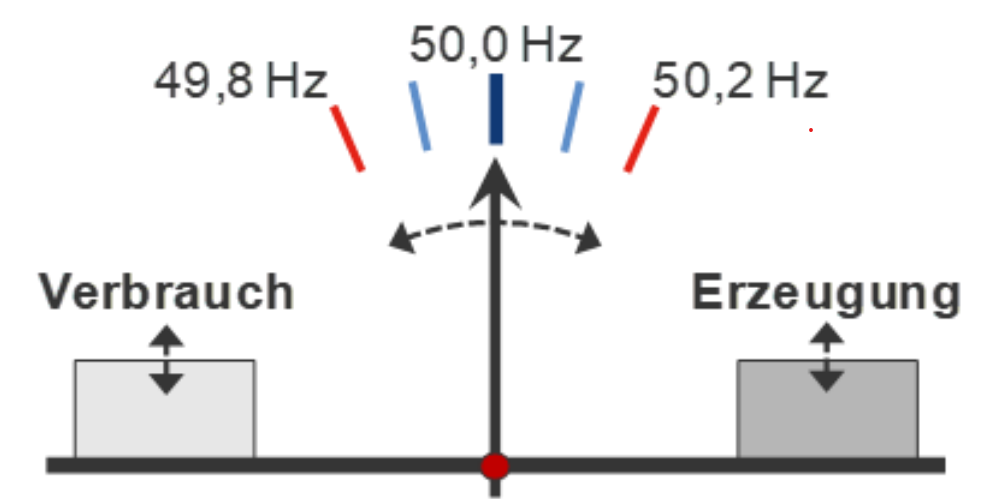
\includegraphics[width=6cm]{Abbildungen/Sollfrequenz.png}
    \caption{Frequenzschwankungen durch Ungleichgewicht von erzeugter und verbrauchter Leistung~\parencite{cronenberg_beschreibung_nodate}}\label{Gleichgewicht}
\end{figure}

Die benötigte Energie ist dabei unterteilt in Momentanreserve, Primärreserve, Sekundärreserve 
und Tertiärreserve.
Die Momentanreserve, welche geringe Frequenzabweichung direkt ausgleichen soll, wird im deutschen Verbundnetz
durch die Schwungmasse der Kraftwerks-Synchronmaschinen bereit gestellt.
Die Primärreserve hingegen greift erst ab einer Abweichung von $20\ mHz$ und musss nach spätestens 30 Sekunden
sowie für mindestens 15 Minuten vollständig zur Verfügung stehen.
Hierfür werden heute schon zunehmend Batteriespeicher eingesetzt.
Zusätzlich wird nach 30 Sekunden die Sekundärregelleistung bereit gestellt, welche für eine Stunde verfügbar sein muss.
Nach 15 Minuten wird diese dann von der Tertiärregelreserve abgelöst, welche ebenfalls fürr eine Stunde verfügbar sein muss.
Die beiden letzten Regeleneergie-Kategorien werden in aller Regel von Kraftwerken in Teillast oder Kraftwerken mit kurzen Anfahrzeiten
erzeugt.
Zuletzt werden einzelne Netzabschnitte vom Netz getrennt um einen Zusammenbruch des Bilanzkreises zu vermeiden.
Dieses Vorgehen bleibt allerdings die äußerste Maßnahme und soll in aller Regel vermieden werden.

Für ein Inselnetz besteht nicht die Möglichkeit Teilnetze abzutrennen. 
Im schlimmsten Fall müssen einzelne Verbraucher und Erzeuger vom Netz getrennt werden um einen stabilen Betrieb zu sichern.
Um das weitestgehend zu vermeiden, ist eine Überdimensionierung von Erzeugern und Speichern meist das Mittel der Wahl.
Große Speicher zur Primärreserve bilden dabei einen wichtigen Grundpfeiler, wobei gerade Batteriespeicher 
auf Grund ihres schnellen Regelverhaltens in Frage kommen~\parencite{Itschner}.

Zusätzlich sollen hier neben der klassischen Regelreserve der Vollständigkeit halber die Regelleistungsprodukte \texttt{Enhanced Frequency Response}
(EFR) und \texttt{Virtuelle Schwungmasse} (VSM) erwähnt werden.
Diese sind zwar noch nicht in den deutschen Markt integriert, könnten aber in der Zukunft eine wichtige Rolle spielen.

EFR setzt dabei schon vor der Primärreserve ein und stellt die volle Regelenergie ab spätestens 1 Sekunde bereit.
Damit füllt EFR die Lücke die durch die fehlenden großen Synchronmaschinen entsteht und wird z.B. bereits vom 
größten britischen Netzbetreiber eingesetzt.
Durch die hohen Anforderungen an die Einschaltzeiten bieten sich auch für diesen Einsatz vor allem
Lithium-Ionen-Batterien an~\parencite{mantar_gundogdu_battery_2018}.

Beim Prinzip der VSM wird versucht die Frequenzstabilität zu verbessern indem Speicher an das Netz angeschlossen werden
die im Wesentlichen das Trägheitsverhalten von mechanischen Schwungmassen in Generatoren imitieren.
Gerade kleiner Inselnetzen welche vor allem durch regenrative Energien betrieben werden könnten hierdurch profitieren.
Auf Grund des kontinuierlichen Energieaustausches mit dem Netz bieten sich für die Umsetzung von VSM-Anlagen vor allem
Speicher mit hoher Lebensdauer und Zyklenzahl an~\parencite{boxleitner_virtuelle_2009}.

\subsection{Rahmenbedingung und Bestimmungen}

In Deutschland sind die Übertragungsnetzbetreiber dafür verantwortlich die Frequenz innerhalb ihrer Regelzone auf möglichst
50 Hz zuhalten.
Dafür stehen Ihnen die oben genannten Regelreserveprodukte zur Verfügung, welche von unterschiedlichen Teilnehmern
des Regelreservemartkes bereit gestellt werden können.
Die verschiedenen Übertragungsnetzbetreiber kooperieren dabei im Netzregelverbund, welcher ein Konzept darstellt,
die Vorhaltung von Regelreserve technisch und wirtschaftlich zu optimieren.
In Zukunft ist ein solches, stark koordiniertes Vorgehen auch auf zentraleuropäischer Ebene geplant.

Im Folgenden sollen die Anforderungen und Bestimmungen zu den einzelnen in Deutschland zugelassenen Regelreserveprodukten 
zusammengefasst werden.

\begin{itemize}
    \item Primärreserve oder \texttt{Frequency Containment Reserve} (FCR) ist darauf ausgelegt die Netzfrequenz möglichst schnell zu stabilisieren. Dafür wird die FCR proportional zur Abweichung der Frequenz von ihrem Sollwert geregelt. Sie wird automatisch bei Abweichungen über 10 mHz aktiviert und soll spätestens nach 30 Sekunden vollständig zur Verfügung stehen.
    \item Sekundärreserve oder \texttt{automatic Frequency Restoration Reserves} (aFRR) löst die Primärreserve ab indem sie die Frequenzabweichung vollständig ausgleicht. Die aFRR ist dafür als Proportional-Integral-Regelung umgesetzt und ist nicht nur abhängig von der Netzfrequenzabweichung sondern zusätzlich vom Leistungsaustausch zwischen den Bilanzkreisen.
    \item Tertiärreserve oder \texttt{manual Frequency Restoration Reserve} (mFRR) löst die aFRR bei länger anhaltenden Störungen ab. Sie ist daher nicht automatisch aktiviert und muss erst innerhalb von 15 Minuten vollständig aktivierbar sein.
\end{itemize}

Zusätzlich sind in \parencite[]{Verordnung} folgende FCR-spezifischen Anforderungen genannt:
\begin{itemize}
    \item [\glqq{} a] die FCR-Aktivierung darf nicht künstlich verzögert werden und muss nach einer Frequenzabweichung so bald wie möglich beginnen;
    \item [b] im Falle einer Frequenzabweichung von mindestens 200 mHz sind spätestens nach 15 Sekunden mindestens 50 \% der vollständigen FCR-Kapazität bereitzustellen;
    \item [c] im Falle einer Frequenzabweichung von mindestens 200 mHz sind spätestens nach 30 Sekunden 100 \% der vollständigen FCR-Kapazität bereitzustellen;
    \item [d] im Falle einer Frequenzabweichung von mindestens 200 mHz muss die Aktivierung der vollständigen FCR-Kapazität im Intervall von 15 bis 30 Sekunden mindestens linear ansteigen, und 
    \item [e] im Falle einer Frequenzabweichung von weniger als 200 mHz muss die entsprechende aktivierte FCR-Kapazität mindestens proportional zu dem unter den Buchstaben a bis d genannten gleichen Zeitverhalten sein.\grqq{}
\end{itemize}

\begin{figure}[h!]
    \centering
    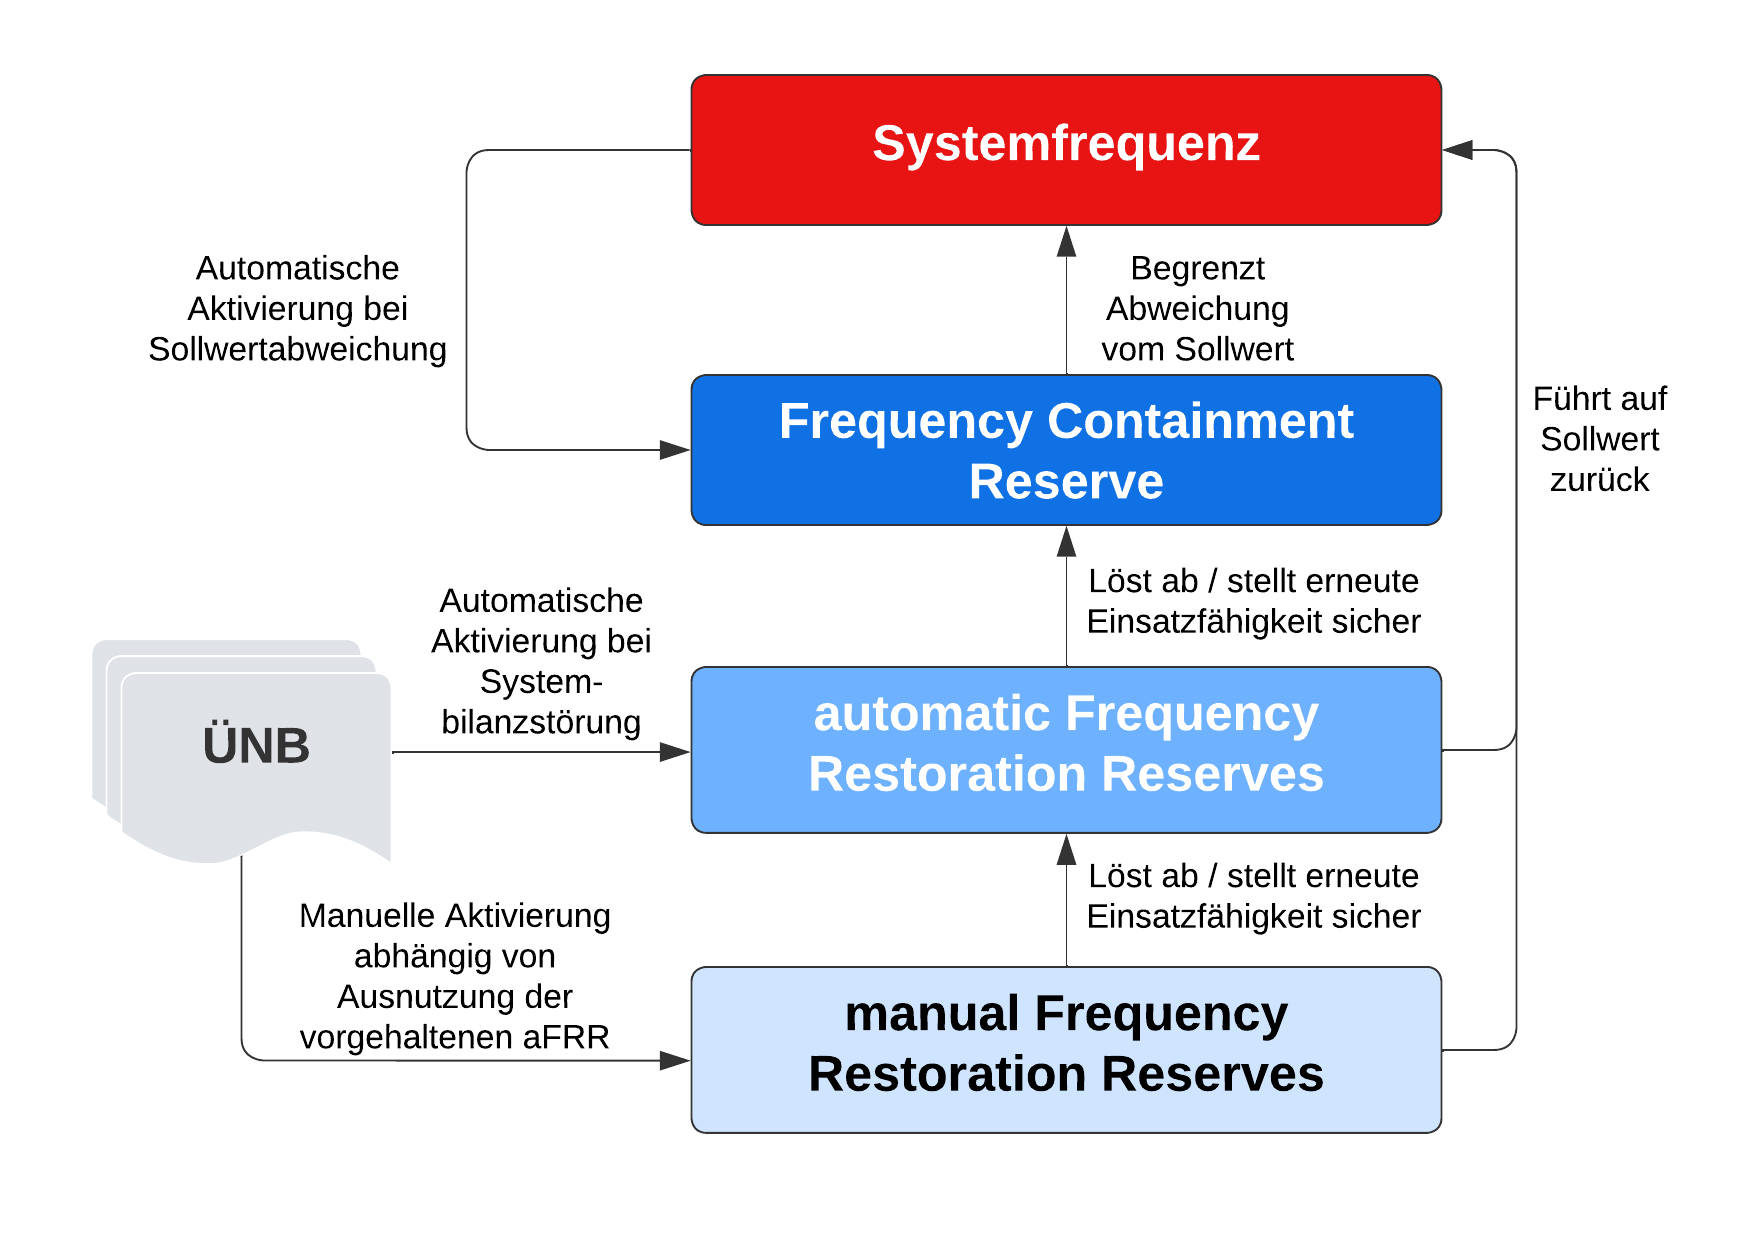
\includegraphics[width=11cm]{Abbildungen/_Flussdiagramm (1).png}
    \caption{Überblick über die verschiedenen Regelreserveprodukte aus~\parencite{cronenberg_beschreibung_nodate}}\label{Fluss}
\end{figure}


\subsection{Betriebsstrategien zu Batteriespeichern}\label{Betriebsstrategien}

Für die Modelle und Simulationen in dieser Projektarbeit werden von den, im letzten Paragraphen beschriebenen Regelreserveprodukten
im Wesentlich zwei genauer betrachtet.
Einerseits die Primärreserve oder FCR und andererseits die EFR, die zwar bisher von deutschen Übertragungsnetzbetreibern nicht genutzt wird
aber gerade für ein Inselnetz wie das hier geplante, eindeutige Vorteile bietet.

Betrachtet man die Anforderungen an diese beide Methoden der Regelleistungsbereitstellung, so kommen vor allem
Batteriespeicher und insbesondere Lithium-Ionen-Batterien für eine Auswahl der Speichertechnologien in Frage.
Im Folgenden sollen verschiedene Methoden zur Umsetzung von FCR- und EFR-Speichern mit Hilfe von Batteriespeichern 
diskutiert und vorgestellt werden.

Beim Betrieb von Batteriespeichern zur Bereistellung von Regelleistung ist der limitierende Faktor der Kapazitäten zu bedenken.
Durch den so genannten State of Charge (SOC) kann ausgedrückt werden, wie viel Prozent ihrer Kapazität einer Batterie noch zur Verfügung stehen.
Um möglichst zu jedem Zeitpunkt die Anforderungen an die PCR oder EFR erfüllen zu können ist eine intelligente
SOC-Steuerung daher unerlässlich.

\begin{figure}[h!]
    \centering
    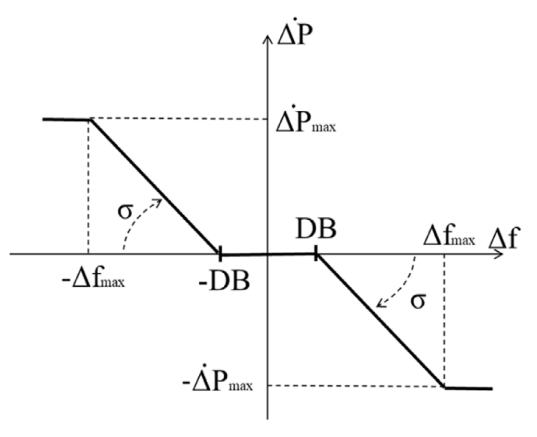
\includegraphics[width=8cm]{Abbildungen/DroopControl.png}
    \caption{Vorgabe der Leistungskurve für PCR-Bereitstellung aus~\parencite[Kap. 3]{noauthor_soc_nodate}}\label{Droop}
\end{figure}

Abbildung~\ref{Droop} zeigt den vorgegebenen Verlauf der Leistungsbereitstellung für PCR-Produkte.
Im letzten Paragraphen wurde bereits beschrieben, dass hierbei ein proportionaler Verlauf zur Frequenzabweichung 
gefordert ist, sobald die Abweichung einen gewissen Grenzwert überschreitet.
Bei einer reinen Umsetzung dieser Kurve mit Hilfe von Batterien, würde unweigerlich, ein Ungleichgewicht von 
Frequenzerhöhungen und Frequenzeinbrüchen dazu führen, dass die Batteriespeicher irgendwann keine Leistung mehr
zur Verfügung stellen können.

Um das zu vermeiden wird in~\parencite[]{noauthor_soc_nodate} unter anderem eine sogenannte Dead band strategy beschrieben.
Der Grundgedanke sieht vor, dass ein Ziel-SOC von z.B. 50 \% festgelegt wird und anschließend während Phasen mit 
Frequenzabweichung innerhalb der Grenzwerte Leistung ausgetauscht werden kann, um den optimalen SOC zu erreichen.
Die maximale Leistung die dabei genutzt werden darf, ist in Deutschland beschränkt.
So darf über 50 Hz keine Leistungsabgabe mehr erfolgen und unter 50 Hz keine Leistungsaufnahme,
sofern allerdings innerhalb des Totbands dem linearen Verlauf der Leistungskurve gefolgt wird,
ist ein Leistungsaustausch zulässig~\parencite[]{marchgraber_modellierung_2019}.

\begin{figure}[h!]
    \centering
    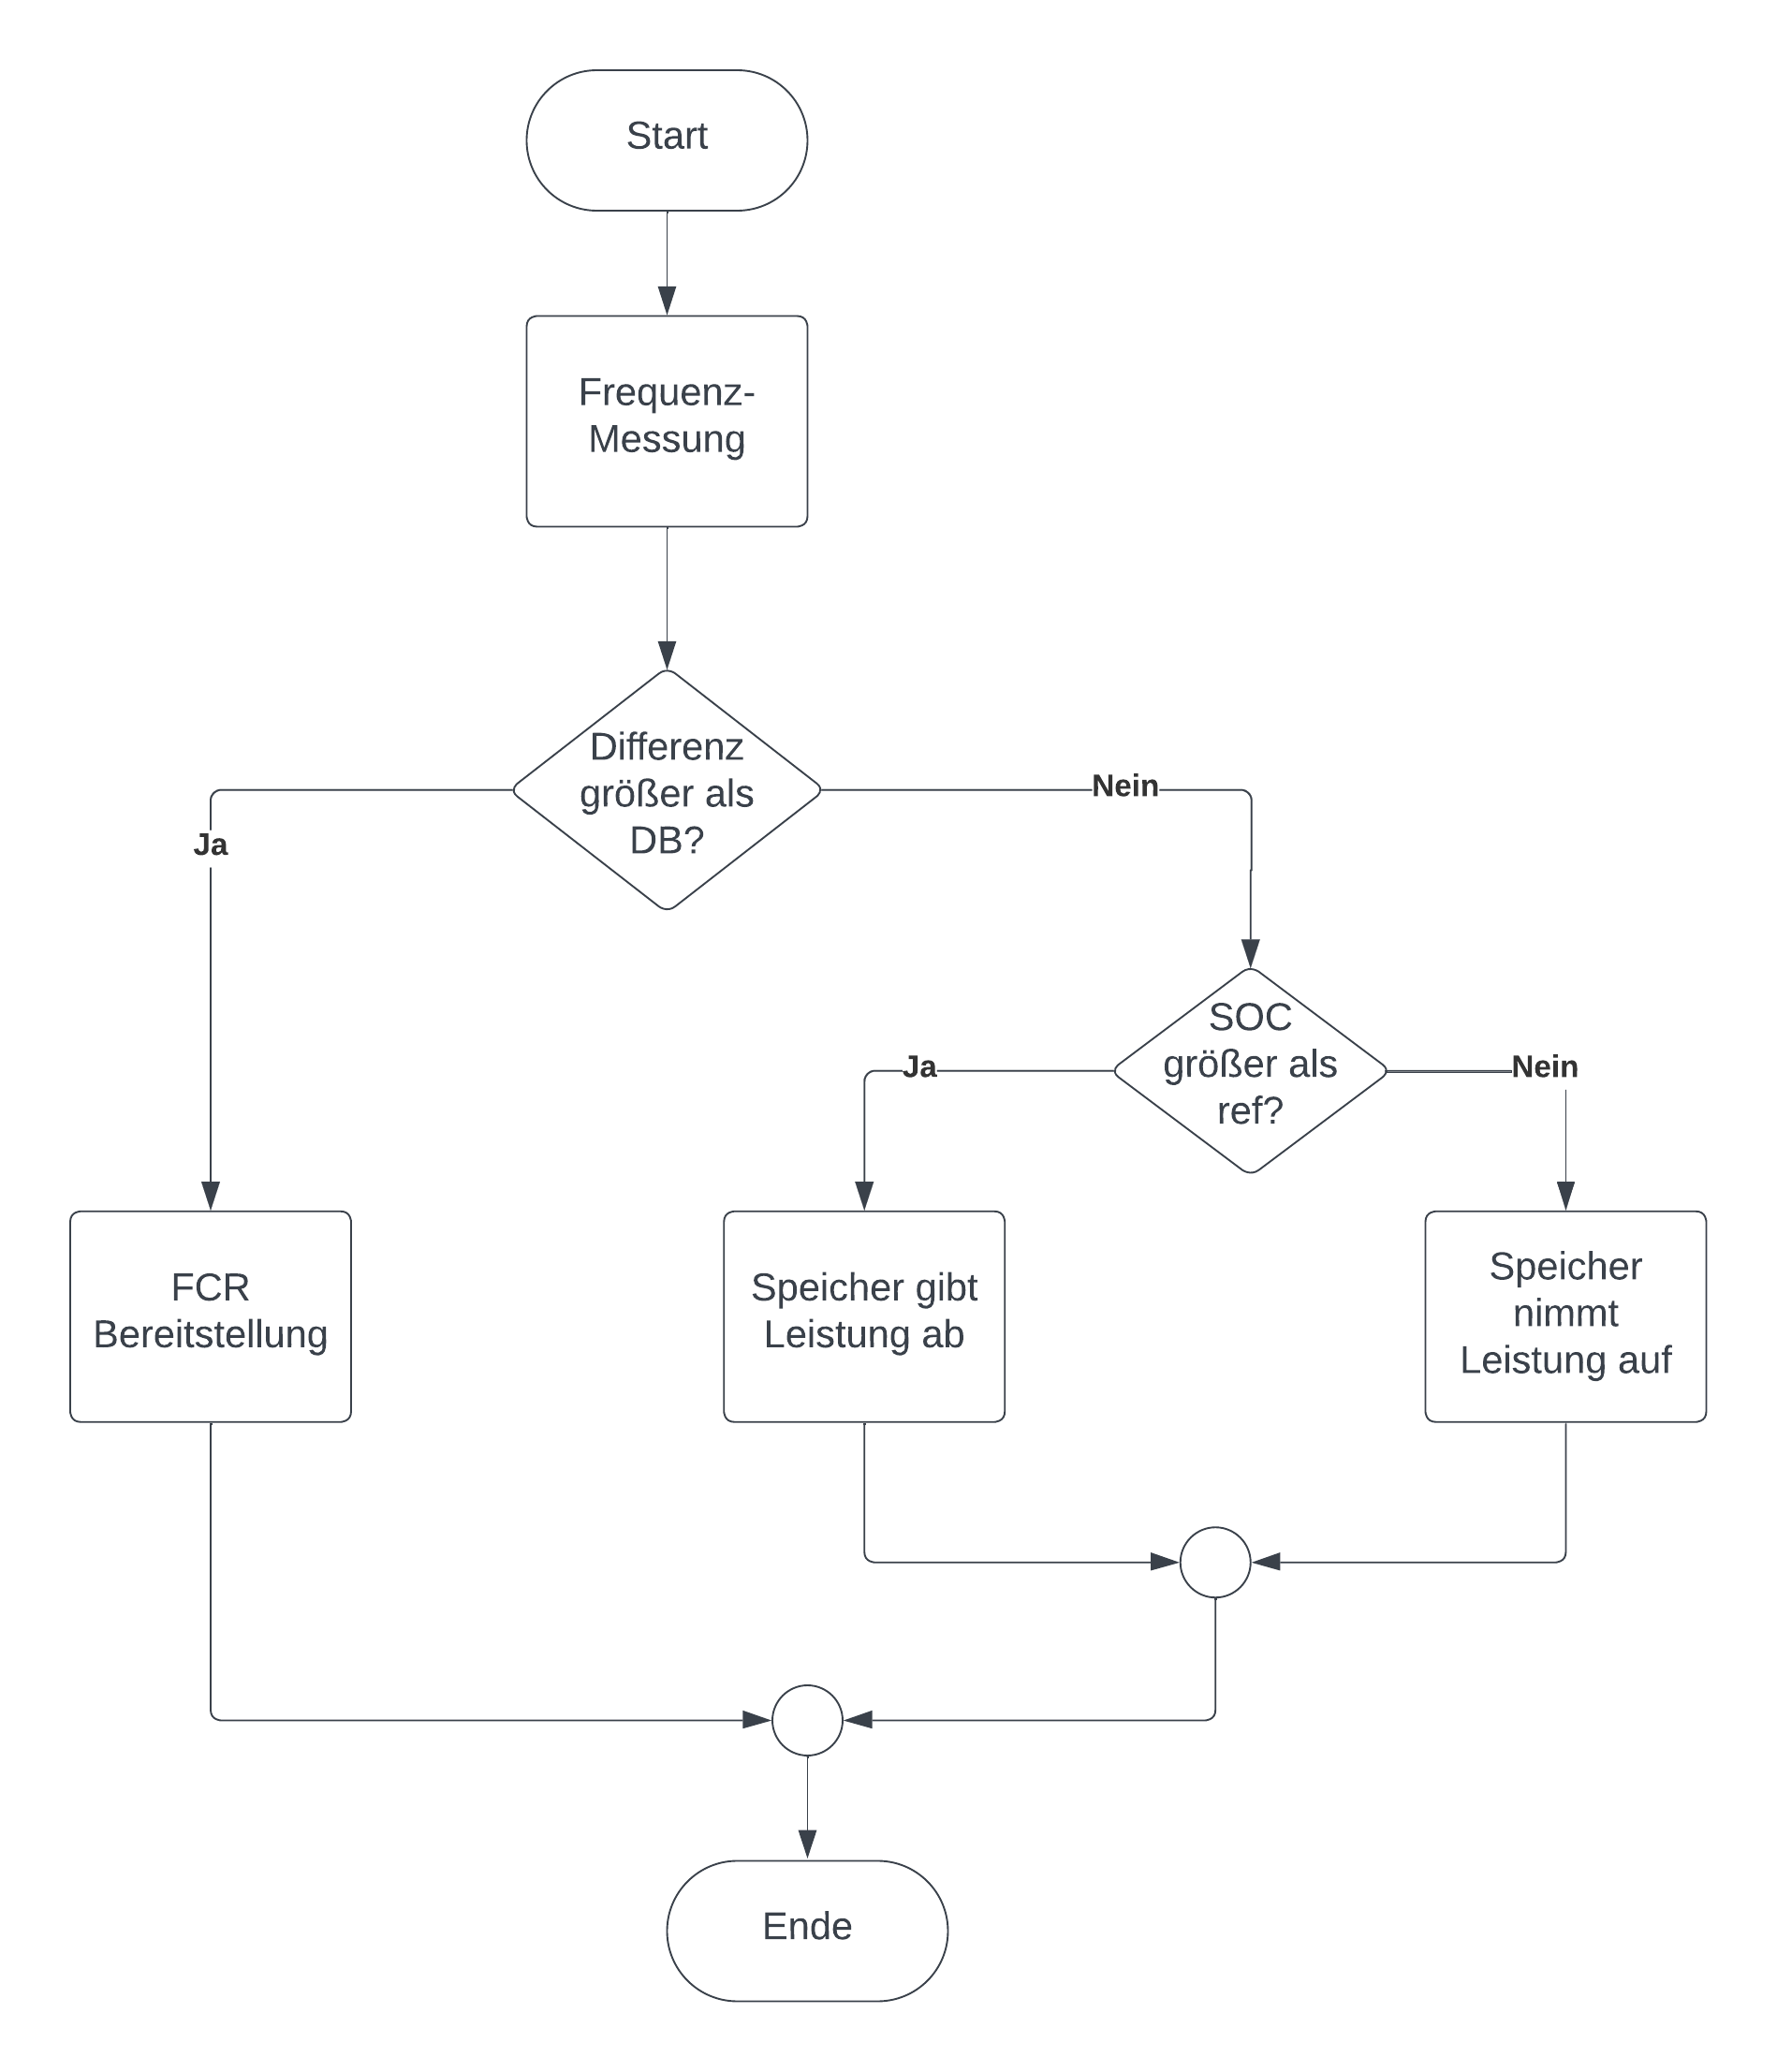
\includegraphics[width=8cm]{Abbildungen/DBFlow.png}
    \caption{Flussdiagramm zur Deadband-Strategie aus~\parencite[]{noauthor_soc_nodate}}\label{FlowPCR}
\end{figure}

Abbildung~\ref{FlowPCR} zeigt ein Flussdiagramm zur Ausnutzung des Totbands.
Ein Nachteil dieser Methode bleibt allerdings, dass nur bei geringen Abweichungen der Netzfrequenz und nur mit begrenzter 
Geschwindigkeit der Ziel-SOC hergestellt werden kann. 
Eine Überdimensionierung des Speichers, um auch bei längeren Störungen Regelleistung bereitstellen zu können, bleibt
also erforderlich.
Für das dreiphasige Modell dieser Projektarbeit soll diese Methode umgesetzt werden. 
Das Vorgehen dafür wird in Kapitel~\ref{Speicher} erläutert.

Ein weiterer Ansatz ist die Festlegung von Leistungssollwerten in Abhängigkeit vom aktuellen SOC.
Für dieses Vorgehen wird die Leistungskurve der Droop-Control um den Leistungssollwert $\Delta P_{SOC}$ nach oben
oder nach unten erweitert je nachdem ob der SOC unter oder über dem festgelegten Zielwert liegt.

\begin{figure}[h!]
    \centering
    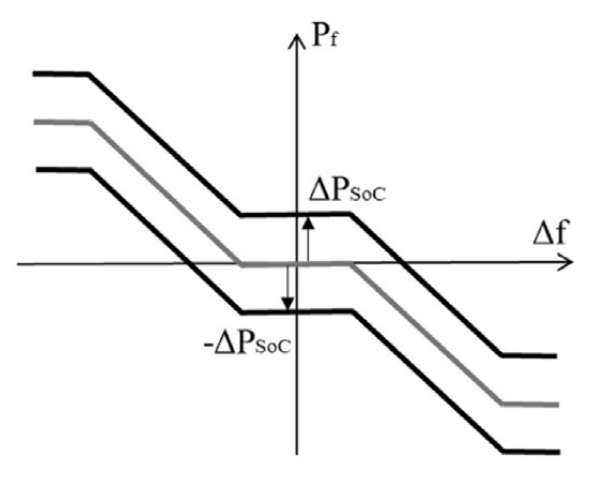
\includegraphics[width=7cm]{Abbildungen/DroopErweitert.png}
    \caption{SOC-Wiederherstellung mit Leistungssollwerten aus \parencite[]{noauthor_soc_nodate}}\label{Droopplus}
\end{figure}

Abbildung~\ref{Droopplus} zeigt den resultierenden Leistungsverlauf.
Dabei muss die maximale Leistungsaufnahme bzw. -abgabe der Batterie berücksichtigt werden und die Vorgaben der
Übertragungsnetzbetreiber müssen eingehalten werden.
Ein sehr ähnlicher Ansatz wird auch in \parencite[]{mantar_gundogdu_battery_2018} für den EFR-Einsatz genutzt.
Dort wird allerdings noch einmal hervorgehoben, dass ein starrer Ziel-SOC von z.B. exakt 50 \% die 
Anzahl der Lade- bzw. Entladezyklen erhöht und sich damit negativ auf die Lebensdauer der Batterien auswirkt.
Für die praktische Umsetzung sollte also ein SOC-Bereich von z.B. 45 \% bis 55 \% angestrebt werden.

\chapter{Stand der Technik}

Bei der Simulation des Inselnetzes liegt der Fokus hinsichtlich des Stands der Technik insbesondere auf zwei Gebieten. Zum einen handelt es sich um Inselnetze als Ganzes. Dabei werden verschiedene Fragen beantwortet, u.a. welche Inselnetze in der Realität existieren oder existierten und warum dies so ist. Zum anderen werden potentielle Speicherarten betrachtet und auf das zu simulierende Inselnetz bezogen analysiert. Ziel ist es, eine technisch und wirtschaftlich realistische Betrachtung zu ermöglichen.

\section{Inselnetze}

Als Inselnetz, auch autonomes Netz genannt, wird ein Stromnetz bezeichnet, welches nur ein kleines Gebiet versorgt und keinen Anschluss an andere Stromnetze besitzt. 
Es stellt das Gegenstück zum Verbundnetz dar, welches aus mehreren kleinen, synchronisierten Netzen besteht\cite{energielexikon}. 
Es gibt verschiedene Gründe, ein Inselnetz aufzubauen. Häufige Anlässe, ein Inselnetz aufzubauen, bestehen in der geographischen isolierten Position
oder politischen Lagen von Gebieten, für die eine Stromversorgung aufrechterhalten werden soll. 
Historische Beispiele hierfür sind die Nordseeinsel Helgoland, welche bis 2009 durch Dieselgeneratoren Strom ihre Stromversorgung sicherstellte\cite{merkur} und West-Berlin, 
dessen externe Stromversorgung durch die Blockade der sowjetischen Besatzungszone 1948 binnen vier Tagen vollständig gekappt wurde\cite{berlinstreet}. 
Auch heutzutage gibt es noch Inselnetze, beispielsweise das der 30.000-Einwohner Stadt Fairbanks im US-Bundesstaat Alaska\cite{iseralaska} oder 
der Färöer-Inseln\cite{cigre-article}. 
Letzteres ist für den Aufbau des Netzes der fiktiven Kommune von größter Relevanz, da dieses momentan entwickelt wird, 
um eine Stromversorgung mit ausschließlich erneuerbaren Energien zu ermöglichen\cite{trondheim-thesis}. 
Dabei ist das Ziel Wind als primäre Energiequelle zu nutzen, was auch für das vorliegende Projekt zutrifft. Bei einer Einwohnerzahl von 54.000\cite{statista-population} und dazugehöriger Industrie und Infrastruktur liegt ein höherer Strombedarf als für dieses Projekt vor, jedoch bewegt dieser sich voraussichtlich in einer ähnlichen Größenordnung, sodass der Aufbau, untersuchte Parameter und tiefere Analysen für das fiktive Projekt relevant sind.
Weitere Inselnetze werden für beispielsweise für Flugzeuge, Schiffe oder sensible Infrastruktur, wie Krankenhäuser oder militärische Einrichtungen, betrieben. 
Diese werden nicht weiter betrachtet.
Ein Inselnetz einer Kommune kann vom Aufbau generell leicht skizziert werden. 
Es besteht im vorliegenden Fall aus einem Verteilverbund  aus Stromerzeugern und -verbrauchern, als auch Speichersystemen. 
Das Netz wird durch verschiedene technische Geräte, beispielsweise Trafos, und einer Regelung gestützt. 

\begin{figure}[h!]
    \centering
    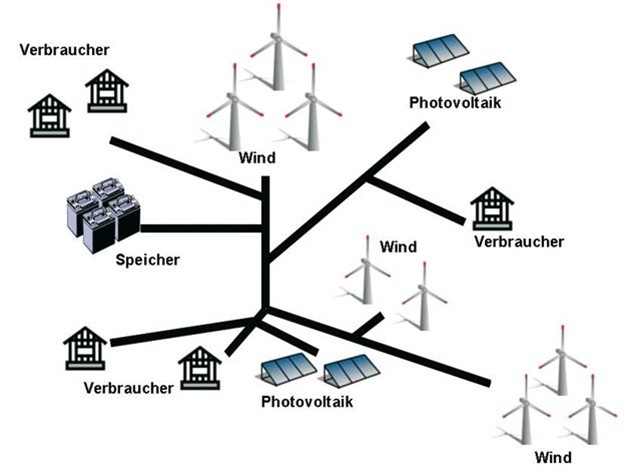
\includegraphics[width=14cm]{Abbildungen/StandDerTechnikAbb1.jpg}
    \caption{Skizze Inselnetz\cite{forwind}}\label{fig:Skizze_Inselnetz}
\end{figure}

Zu den regenerativen Stromerzeugern, welche genutzt werden können, zählen Windkraft, wobei zwischen On- und Off-Shore unterschieden wird, 
Photovoltaik, Wasserkraft und Geothermie. Die Auswahl der Stromerzeuger nach den lokalen Gegebenheiten. 
Auf den Färöer-Inseln bietet sich aufgrund der Lage insbesondere Windkraft , sowohl On-Shore als auch Off-Shore, an. 
Darüber hinaus wurde die Nutzung von Wasserkraft in Form von Gezeitenkraftwerken geprüft\cite{trondheim-thesis}. 
Auch Geothermie und Photovoltaik spielen eine Rolle. Für deutsche Kommunen sind diese Stromerzeuger auch relevant, wobei sich 
geothermische Kraftwerke ausschließlich in Süddeutschland finden lassen. 
Die Stromverbraucher setzen sich auf kommunaler Ebene aus einer Mischung aus Wohn- und Nichtwohngebäuden als auch gegebenenfalls industrieller Abnehmer zusammen. 
Als Speichersysteme kommen z. B. Batterien in Frage. In der Praxis werden häufig Lithium-Ionen oder Redox-Flow-Batterien genutzt. 
Solche Speicher, insbesondere auf Gebäudeebene, können diese zu sogenannten Prosumern  machen und schon heute ein relevanter Faktor bei der Netzregelung sein. 
Darüber hinaus fallen Wärme-, Druckluftspeicher, Pumpspeicherwerke und die Zwischenlagerung als Wasserstoff unter nutzbare Speichersysteme bei Nutzung erneuerbarer Energien. 
Zur kurzzeitigen Speicherung von Strom zur Netzstabilität ist außerdem die Nutzung von Spulen, Kondensatoren oder Schwungmassenspeichern möglich. 
Inselnetze haben im Vergleich zu Verbundnetzen eine Reihe von Vor- und Nachteilen. 
Sie können autonom operieren und unterliegen einer lokalen Kontrolle. 
Dadurch wird die Anpassung der Energieproduktion und -verteilung an die Bedürfnisse der Verbraucher einfacher. 
Außerdem sind Transportverluste und die Komplexität des Systems deutlich geringer als bei Verbundnetzen. 
Dagegen steigen die Stromerzeugungskosten, was die Wirtschaftlichkeit des Inselnetzes erschwert. 
Ein weiterer Nachteil ist, dass eine Kommune oder Inselgruppe über geographisch begrenzte Ressourcen verfügt. 
Erneuerbare Energien, beispielsweise Photovoltaik und Windkraft, sind limitiert einsetzbar und volatil gegenüber Wetterschwankungen. 
Bei anhaltender Dunkelflaute oder einer Beschädigung des Inselnetzes ist die Versorgungssicherheit eines Solchen, wie dem der Färöer-Inseln, unmittelbar gefährdet.
Insgesamt sind solche Inselnetze meist darauf ausgelegt, einen Überschuss an elektrischer Energie zu produzieren. 
Für das Stromnetz der Färöer-Inseln wurde 2021 berechnet, dass für die Tagesproduktion an Strom Kapazitäten von 224% für Wind, 105 % für PV mit 8-9 Tage Speicherkapazität gerechnet werden müssen, um eine Versorgung von 87 % aus erneuerbaren Energien zu gewährleisten\cite{researchgate-paper}.  
 
\begin{figure}[h!]
    \centering
    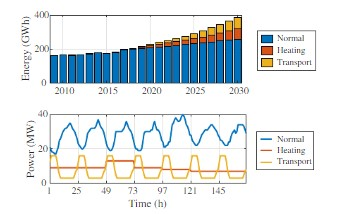
\includegraphics[width=14cm]{Abbildungen/StandDerTechnikAbb2.jpg}
    \caption{Stromprognose und Lastverläufe Färöer-Inseln, Stand 2021\cite{trondheim-thesis}}\label{fig:Stromprognose_und_Lastverläufe}
\end{figure}

In solchen Prognosen ist es außerdem wichtig, Prognosen des Strombedarfs für mehrere Jahre in die Zukunft zu berücksichtigen (s. Abbildung 2). 
Die Lastverläufe sind außerdem in Kombination mit fluktuierender Stromerzeugung von hoher Relevanz für Regelung und Speicher. 
Dabei ist eine wochenbezogene Betrachtung üblich.

\section{Speicher}

Die Speicherung von Strom spielt in der Simulation eine zentrale Rolle. 
Um den Aufbau von realistischen Speichersystemen im fiktiven Inselnetz zu ermöglichen, 
ist ein Blick auf den Stand der Technik solcher Speichertechnologie notwendig. 
Im Fokus stehen dabei Be- und Entladeverhalten von genutzten Batterien, da deren Verhalten fundamental für Be- und Entladestrategien ist. 
Außerdem werden weitere Speichertechnologien genauer betrachtet, um den Nutzen ihres Einsatzes in der Simulation abzuschätzen. 
Eine Gegenüberstellung dieser Technologien nach heutigem Stand von Ausspeicherdauer zu Speicherkapazität in 
logarithmischer Skalierung kann nachfolgender Abbildung entnommen werden.

\begin{figure}[h!]
    \centering
    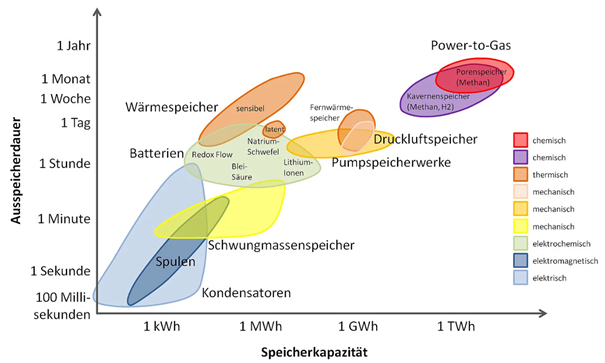
\includegraphics[width=14cm]{Abbildungen/StandDerTechnikAbb3.png}
    \caption{Speichertechnologien Übersicht\cite{eespeicher}}\label{fig:Speichertechnologien_Übersicht}
\end{figure}
 
Batteriespeicher gehören zu den am häufigsten genutzten Speicherformen für Inselnetze. 
Eine genauere Betrachtung der verschiedenen Batterietypen nach ihrem Stand der Technik bietet sich an. 
Relevant sind dabei insbesondere der Wirkungsgrad, die Lebens- bzw. Zyklenlebensdauer, 
der Temperaturbereich in welchem die Batterien arbeiten können und die Kosten.


%\hskip-4.0cm\begin{table}{\textwidth}{@{\extracolsep{\fill}}rclp{4cm}}
\begin{table}    
    \centering
    \caption{Gegenüberstellung Batteriespeicher Stand der Technik}
    \label{tab:Gegenüberstellung_Batteriespeicher_Stand_der_Technik}
    \begin{tabular}{p{2.2cm}|p{2.2cm}|p{2.2cm}|p{2.2cm}|p{2.2cm}|p{2.2cm}|p{2.2cm}|}
        %\toprule
        \textbf{Batterietyp} & \textbf{Energie-dichte [Wh/kg]} & \textbf{Wirkungs-grad [\%]} & \textbf{Lebensdauer [Jahre]} & \textbf{Zyklenlebens-dauer [-]} & \textbf{Temperatur-bereich [°C]} & \textbf{Kosten [€/kWh]} \\
        %\midrule
        Blei-Säure & 25-40 & 80-90 & 3-12 & 50-2.000 & -20 bis +50 & 100-300 \\
        Lithium-Ionen & 70-260 & 90-95 & Bis zu 15 & >2.000 & 0 bis +40 & 92 \\
        Natrium-Ionen & 140-160 & 90 & k.A. & >50.000 & -20 bis +45 & 60\cite{energieexperten} \\
        Nickel-Metallhybrid & 80 & 70-90 & Bis zu 10 & 500 (i.L.) & Über 0°C & 150 – 300* \\
        Natrium-Schwefel & 218 & 75-85 & Ca. 10 & 2.500 (i.L.) & +300 bis +350 & 200 – 400* \\
        Redox-Flow (Vanadium) & 10-85 & 70-80 & >15 & >15.000 & 0 bis +40 & 200 – 500* \\
        %\bottomrule
    \end{tabular}
\end{table}

*grobe Schätzung

%\begin{table}[htbp]
%    \centering
%    \caption{Gegenüberstellung Batteriespeicher Stand der Technik}
%    \begin{tabular}{lcccccc}
%    \label{tab:Gegenüberstellung_Batteriespeicher_Stand_der_Technik}
%        \toprule
%        \textbf{Batterietyp} & \textbf{Energiedichte [Wh/kg]} & \textbf{Wirkungsgrad [\%]} & \textbf{Lebensdauer [Jahre]} & \textbf{Zyklenlebensdauer [-]} & \textbf{Temperaturbereich [°C]} & \textbf{Kosten [€/kWh]} \\
%        \midrule
%        Blei-Säure & 25-40 & 80-90 & 3-12 & 50-2.000 & -20 bis +50 & 100-300 \\
%        Lithium-Ionen & 70-260 & 90-95 & Bis zu 15 & >2.000 & 0 bis +40 & 92 \\
%        Natrium-Ionen & 140-160 & 90 & k.A. & >50.000 & -20 bis +45 & 60\cite{energieexperten} \\
%        Nickel-Metallhybrid & 80 & 70-90 & Bis zu 10 & 500 (i.L.) & Über 0°C & 150 – 300* \\
%        Natrium-Schwefel & 218 & 75-85 & Ca. 10 & 2.500 (i.L.) & +300 bis +350 & 200 – 400* \\
%        Redox-Flow (Vanadium) & 10-85 & 70-80 & >15 & >15.000 & 0 bis +40 & 200 – 500* \\
%        \bottomrule
%    \end{tabular}
%\end{table}
%*grobe Schätzung

Unter Betrachtung der verglichenen Eigenschaften von genutzter Batteriespeicher die meisten betrachteten Technologien 
aus der Auswahl für ein Inselnetz heraus. Blei-Säure-Batterien sind für die benötigte Speicherkapazität unwirtschaftlich. 
Nickel-Metallhybrid-Batterien sind über alle Eigenschaften hinweg Lithium-Ionen-Batterien unterlegen und werden durch ebendiese momentan ersetzt. 
Da Natrium-Ionen-Batterien eine deutlich geringere Energiedichte haben, eignen sie sich 
als stationäre Batterie-Speicherkraftwerke nicht für Wind- und Solarenergie nicht. 
Bei Natrium-Schwefel-Batterien liegt bei der vorliegenden Anwendung das Hauptproblem im nutzbaren Temperaturfenster. 
Die hohen Temperaturen von 300 bis 350°C müssen gehalten werden, wodurch sie als Speicher bisher nur 
für Großspeicher zur Netzstabilisierung Anwendung gefunden haben. 
Als realisierbare Speicher bleiben Lithium-Ionen- und Redox-Flow-Batterien übrig. 
Eine tiefere Analyse folgt.

\subsection{Lithium-Ionen-Batterien}

Bei Lithium-Ionen-Batterien handelt es sich um die am häufigsten genutzte Art von Batteriespeichern. 
Dabei können diese sowohl als kleine stationäre Speicher mit einstelliger kWh-Kapazität in Prosumern, 
beispielsweise Haushalten mit PV-Anlage, oder als Großspeicher im Kapazitätsbereich von mehreren MWh genutzt werden.
Lithium-Ionen-Batterien erreichen mit bis zu 95 \% den höchsten Wirkungsgrad unter allen serienmäßigen Speicherarten. 
Darüber hinaus haben sie mit bis zu 260 Wh/kg auch die höchste Energiedichte. Die Lebensdauer von bis zu 15 Jahren 
und bis zu über 2.000 Zyklen ist vergleichsweise durchschnittlich. 
Das Operationsfenster von 0 bis 40°C ist befindet sich über den Großteil des Jahres im Rahmen der Außentemperaturen 
in Deutschland. Die Selbstentladung pro Monat bei 20°C liegt bei etwa 4 \%\cite{uni-lecture}.
Risiken bei Lithium-Ionen-Batterien liegen bei Fehlfunktionen der Lade-/Entladeelektronik oder durch Überhitzung. 
Resultierend können Feuer entstehen, deren Löschung mit herkömmlichem Löschmittel für die Feuerwehr schwierig ist.
Anwendungsbeispiele für Lithium-Ionen-Batterien als Großspeicher sind 6 und 18 MWh auf Jeju Island, 
Südkorea oder in der Automobilindustrie die Tesla-Batterie. Der Marktanteil liegt von Lithium-Ionen-Batterien liegt bei über 95\%.
Perspektivisch könnten Lithium-Ionen-Batterien von Natrium-Ionen-Batterien abgelöst werden. 
Diese sind aber bisher defizitär hinsichtlich ihrer Energiedichte, jedoch prinzipiell günstiger und thermisch robuster. 

\subsection{Redox-Flow-Batterien}

Der Aufbau einer Redox-Flow-Batterie besteht aus mindestens zwei Halbzellen. Dies ermöglicht verschiedene Materialpaarungen. 
Mögliche Materialpaarungen sind u. a. Vanadium/Vanadium, Chrom/Eisen oder Zink/Bromid. 
Da die Auswahl der Materialpaarung einen wesentlichen Einfluss auf die Energiedichte hat, 
hat sich als meistverbreitete Technologie Vanadium/Vanadium durchgesetzt. 
Der Wirkungsgrad von Redox-Flow-Batterien liegt bei 80 \%, wird jedoch durch Verluste beim Pumpvorgang des 
Elektrolyts mit 70 bis 75\% erhöht. 
Bei einer Energiedichte von bis zu 85 Wh/kg bei einer Vanadium/Vanadium-Materialpaarung liegt diese deutlich 
unter den Lithium-Ionen-Batterien. Die Lebensdauer einer Batterie kann 15 Jahre und 15.000 Zyklen überschreiten. 
Das Operationsfenster liegt bei 0 bis 40°C und entspricht dem der Lithium-Ionen-Batterie\cite{uni-lecture}. 
Die Selbstentladung pro Monat bei 20°C liegt bei unter 1 \% und ist damit marginal.
Neben der geringeren Energiedichte der Batterien, welche mit einem größeren Platzbedarf im stationären Betrieb eingehen, 
haben Redox-Flow-Batterien einen Faktor der finanziellen Ungewissheit in der Herstellung. 
Dies liegt daran, dass die effizienteste Materialpaarung aus Vanadium besteht, welches als kritischer Rohstoff gilt und 
starken Preisschwankungen unterliegt\cite{cleanthinking}.
Die Technologie der Redox-Flow-Batterien ist weniger gut erforscht als die der Lithium-Ionen-Batterien und wird aktuell stärker erforscht, 
da größeres Potential für Verbesserungen vermutet wird. 
Bereits 2020 wurde an der University of South California eine Anthrachinondisulfonsäure/Eisensulfat-Materialpaarung genutzt, 
mit der Kosten von 54 €/kWh\cite{yang2020redoxflow} erzielt werden konnten. Damit liegt man im Kostenbereich von Natrium-Ionen-Batterien und 
unter Lithium-Ionen-Batterien. Langfristig ist eine kommerzielle Nutzung von Redox-Flow-Batterien als Großspeicher denkbar. 
Ein Pionierprojekt in der Wirtschaft stellt der Bau eines 500 MWh-Redox-Flow-Speichers der LEAG in Boxberg dar. 
Bei diesem Projekt handelt es sich bisher allerdings nur um eine Planung, die bis 2027 umgesetzt werden soll\cite{winfuture-news}.

\subsection{Aufbau von stationären Batteriespeichersystemen}

In einem kommunalen Inselnetz werden häufig ein oder mehrere stationäre Batteriespeichersysteme genutzt. 
In dem hier betrachteten Kapazitätsbereich von mehreren MW spricht man von Großspeichern. 
Im Zuge der Energiewende haben sich Schwerpunkte des Anforderungsprofils solcher Batteriegroßspeicher verändert. 
Wichtige Eigenschaften stellen dabei die Reaktionsgeschwindigkeit, Flexibilität und Zuverlässigkeit solcher Systeme dar.
 
\begin{figure}[h!]
    \centering
    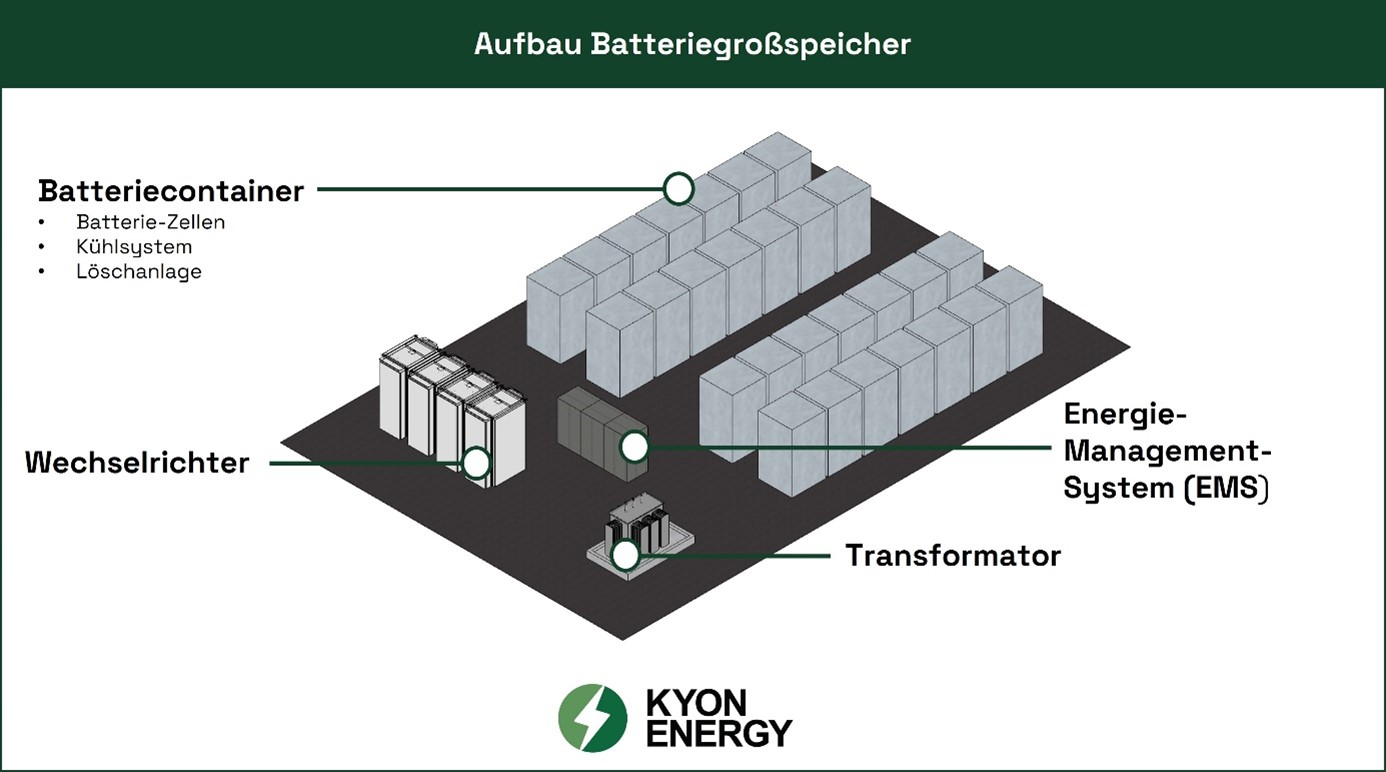
\includegraphics[width=14cm]{Abbildungen/StandDerTechnikAbb4jpg.jpg}
    \caption{Batterispeichersystem Aufbau\cite{kyon-energy}}\label{fig:Batterispeichersystem_Aufbau}
\end{figure}

Ausgangspunkt des Speichers sind die Batteriezellen in einem Container. 
Um die technischen und gesetzlichen Anforderungen zu erfüllen, besitzt jeder Batteriecontainer ein Kühlsystem für die Nutzung und eine Löschanlage für den Brandfall. 
Diese Batteriecontainer können flexibel skaliert werden, also an die Bedürfnisse des Stromnetzes angepasst werden. 
Im Vergleich zu anderen Industrieren wie z.B. der Automobilindustrie, spielt die Energiedichte eine geringere Rolle, als reine Materialkosten. 
Daher werden häufig billigere Zellen aus Lithium-Eisen-Phosphat (LFP), der Alternative mit hoher Energiedichte aus Lithium-Nickel-Mangan-Cobalt (NMC), vorgezogen.

\begin{table}[htbp]
    \centering
    \caption{Auswahl Batteriezellen Großspeicher\cite{poworks-comparison}}
    \label{tab:Auswahl_Batteriezellen_Großspeicher}
    \begin{tabular}{lcccc}
       \toprule
        & \textbf{LFP} & \textbf{NMC} & \textbf{Redox Flow} & \textbf{Redox Flow (Vanadium-Vanadium)} \\
        \midrule
        \textbf{Energiedichte [Wh/kg]} & 230-260 & 130-200 & 10-85 & 85 \\
        \textbf{Kosten [€/kWh]} & 150-250 & 100-200 & 200-500* & 300-500* \\
        \bottomrule
    \end{tabular}
\end{table}

* grobe Schätzung

Da Batterien im Gleichstrom betrieben werden, wird das Batteriesystem durch Wechselrichter vom Netz getrennt. 
Wenn die vorliegenden Energiemengen entsprecht groß sind, bedarf es außerdem eines Transformators, w
elcher den Strom von der Niederspannungsebene auf das gewünschte Spannungsniveau wandelt. 
Wechselrichter und Transformatoren müssen bidirektional verwendbar sein, um Be- und Entladung zu gewähren. 
Die Koordination dieses Vorganges wird durch ein Energie-Management-System (EMS) gewährleistet. 
Dadurch ist es außerdem möglich, Zellen zu überwachen und das System im Problemfall zu schützen\cite{kyon-energy}.



\chapter{Modellbeschreibung}
\section{Erzeuger}
\subsection{Windenergie}
\subsection{Photovoltaik}
\section{Verbraucher}
\section{Speicher}
\section{Netzmodell}
\subsection{Bilanziell}
\subsection{Dreiphasig}


\chapter{Simulationsergebnisse}

\chapter{Auswertung}

\chapter{Fazit}

\chapter{Ausblick}

Der Ausblick umfasst die Betrachtung von möglichen Verbesserungen der Simulationen und technische Entwicklungen, die in naher Zukunft für ein kommunales Inselnetz wirtschaftlich seien könnten.
Eine Zusammenführung der bilanziellen und dreiphasigen Simulation in ein MatLab/Simulink-Modell ist wünschenswert, aufgrund der hohen Simulationszeit des bilanziellen Systems jedoch nur mit unproportionalem Zeitaufwand möglich.
Die simulierte Zeit pro Sekunde sollte dafür vom Verhältnis von ungefähr 1:1 auf 60:1 verbessert werden.
Generell sind bei beiden Simulationsmodellen im Aufbau viele Komponenten und Einflüsse vereinfacht worden. 
Um eine realistischere Simulation zu erhalten, können diese genauer abgebildet werden.
Bei den Stromerzeugern können Photovoltaikanlagen der Simulation hinzugefügt werden.
Anhand von Faktoren wie dem Material der Solarzellen, dem Wirkungsgrad, installierter Leistung, Systemverlust, Neigung und Azimut, sowie Daten für die Solareinstrahlung des Standortes der Kommune kann ein komplexes Modell dieses Erzeugers in MatLab/Simulink erstellt werden\cite{jrcpv}.
Die Implementation des Erzeugers PV würde, da dieser sonneneinstrahlungsabhängig ist, zu einer komplexeren Fluktuation bei der Stromerzeugung im Netz führen. 
Dies hat generellen Einfluss auf das Netz und die Dimensionierung, als auch Be- und Entladestrategien von Speichern.
Weitere erneuerbare Energien, die betrachtet werden können sind Gezeiten- und Wasserkraft (s. Abbildung).
Die Auswahl dieser regenerativen Energiequellen ist jedoch stark von der geographischen Lage des Inselnetzes abhängig.
  
\begin{figure}[h!]
    \centering
    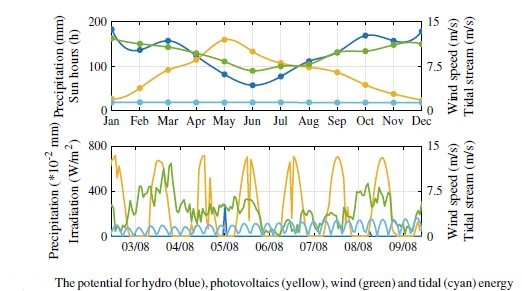
\includegraphics[width=14cm]{Abbildungen/AusblickAbb1.jpg}
    \caption{Betrachtung potentieller erneuerbarer Stromerzeuger für das Fallbeispiel Färöer-Inseln\cite{faroer}}\label{fig:Stromerzeuger_Faroer}
\end{figure}

Außerdem kann die Modellierung eines Prosumers, bestehend aus einem Haus mit Wärmepumpe, PV-Anlage und Speicher, am Netz betrachtet werden.
Die Modellierung ist hierbei komplex und deren Auswirkungen für das Netz können relevant sein.
Ursache dafür ist die Komplexität dieses Subsystem des Inselnetzes.
Bei einem solchen Prosumer liegt ein Zusammenspiel von PV-Anlage und internem Speicher zugrunde.
Für diesen können eigene Be- und Entladestrategien betrachtet werden, die außerdem neben dem allgemeinen Strombedarf des Hauses noch mit dem Strombedarf einer angeschlossenen Wärmepumpe zusammenspielen.
Durch die Abhängigkeit des Heizverhaltens der Wärmepumpe von der Außentemperatur, aus welcher sich der Heizbedarf ermitteln lässt, entsteht zusammenfassend eine in sich komplexe Komponente im Modell.
Ein weiterer Verbrauchsfaktor für ein Inselnetz ist die E-Mobilität.
Hierbei stehen die Betrachtung und ggf. Steuerung des Ladeverhaltens der E-Fahrzeuge im Vordergrund.
Darüber kann die Interkation von privaten E-Fahrzeugen mit privaten Stromspeichern aus dem Modell des beschriebenen Prosumers simuliert werden.
Auch bei den Speichersystemen sind Änderungen implementierbar.
In beiden Modellen werden ausschließlich Batteriespeichersysteme modelliert.
Eine Simulation eines Fernwärmenetzes als auch die Nutzung von Power-to-Gas und Gas-to-Power sind möglicher Erweiterungen für die Modelle.
Die existierenden Batteriemodelle können auch präziser modelliert werden.
Dabei ist die Betrachtung von elektrischen Batteriemodellen ein möglicher Schritt, der es ermöglichen würde, elektrische Phänomene im Netz genauer zu betrachten.
Dadurch können gleichzeitig die Aufgaben von Batteriespeichersystemen umfassender simuliert werden.
Außerdem können in einer erweiterten Simulation auf Dauer weitere relevante Faktoren implementiert werden, beispielsweise ein Peak Shaving Algorithmus.
Eine Darstellung von Redox-Flow-Batteriespeichern findet außerdem auch nicht statt, ist aber möglich und sinnvoll, insbesondere wenn ebendiese wirtschaftlich und technisch eine Alternative zu Lithium-Ionen-Batteriespeichern darstellen.
Für die bilanzielle Simulationen wäre eine Erweiterung der Simulation wünschenswert, bei die Betrachtung von elektrischen Phänomenen allgemein möglich ist. 
Jedoch darf die Simulationsgeschwindigkeit dadurch nicht stark beeinträchtigt werden.
Bei der Modellierung des dreiphasigen Inselnetzes gibt es mehrere Erweiterungsoptionen. 
Die Implementierung einer Ladestrategie für die Windkraftspeicher kann die Qualität der Simulation verbessern.
Darüber hinaus ist in Anbetracht der gewünschten Nutzung von ausschließlich erneuerbaren Erzeugern die Entfernung des Dieselgenerators eine Möglichkeit.
Dies ist allerdings nur umsetzbar, wenn im gleichen Zug eine Implementierung einer Frequenzmessung stattfindet, da der Dieselgenerator essentiell für diese Messung ist.
Darüber hinaus ist die Betrachtung der Blindleistung im Modell implementierbar.
Allgemein können auch Prognosen im Bereich der Strombedarfsermittlung und der Veränderung von Verbrauchern einen Mehrwert für die Modellierung darstellen.
Das liegt daran, dass im Zuge der Abkehr von fossilen Energieträgern insbesondere in den Bereichen Gewerbe, Industrie und Verkehr damit zu rechnen ist, dass ein Großteil des Energiebedarfes in Deutschland und vielen anderen Teilen der Welt auf Dauer durch Strom gedeckt werden soll.
Die resultierende momentane Entwicklung spielt dabei eine ausschlaggebende Rolle und die technische Weiterentwicklung, insbesondere im Bereich der Speichertechnologien, prägt den Aufbau und die Veränderung jedes Stromnetzes.



\pagenumbering{roman}
\appendix


\printbibliography
\end{document}
